%% ----------------------------------------------------------------
%% Thesis.tex -- MAIN FILE (the one that you compile with LaTeX)
%% ---------------------------------------------------------------- 

% Set up the document
\documentclass[a4paper, 11pt, oneside]{Thesis}  % Use the "Thesis" style, based on the ECS Thesis style by Steve Gunn
\graphicspath{Figures/}  % Location of the graphics files (set up for graphics to be in PDF format)

% Include any extra LaTeX packages required
\usepackage[comma]{natbib}  % Use the "Natbib" style for the references in the Bibliography
\bibliographystyle{agsm}
\usepackage{verbatim}  % Needed for the "comment" environment to make LaTeX comments
\usepackage{vector}  % Allows "\bvec{}" and "\buvec{}" for "blackboard" style bold vectors in maths
\hypersetup{urlcolor=blue, colorlinks=true}  % Colours hyperlinks in blue, but this can be distracting if there are many links.
\usepackage{amsmath}
\usepackage{siunitx}
\usepackage{graphicx}

\usepackage{listings}
\usepackage{color}


\definecolor{dkgreen}{rgb}{0,0.6,0}
\definecolor{gray}{rgb}{0.5,0.5,0.5}
\definecolor{mauve}{rgb}{0.58,0,0.82}
\usepackage{fancyhdr}
\usepackage[table]{xcolor}
\usepackage{booktabs,caption}
\usepackage[flushleft]{threeparttable}


\lstset{language=XML,
	aboveskip=3mm,
	belowskip=3mm,
	showstringspaces=false,
	columns=flexible,
	basicstyle={\small\ttfamily},
	numbers=none,
	numberstyle=\tiny\color{gray},
	keywordstyle=\color{blue},
	commentstyle=\color{dkgreen},
	stringstyle=\color{mauve},
	breaklines=true,
	breakatwhitespace=true,
	tabsize=3
}

\usepackage{hyperref}
\hypersetup{
	colorlinks=true,
	linkcolor=blue,
	filecolor=magenta,      
	urlcolor=cyan,
}

\urlstyle{same}




%% ----------------------------------------------------------------
\begin{document}
\frontmatter      % Begin Roman style (i, ii, iii, iv...) page numbering

% Set up the Title Page
\title  {GeiodApp: A Unified Framework for Geoid Computations}
\author{Mohamed Jaafar and Mohamed Yousif}
\addresses  {\groupname\\\deptname\\\univname}  % Do not change this here, instead these must be set in the "Thesis.cls" file, please look through it instead
\date       {\today}
\subject    {}
\keywords   {}

\maketitle
%% ----------------------------------------------------------------

\setstretch{1.3}  % It is better to have smaller font and larger line spacing than the other way round

% Define the page headers using the FancyHdr package and set up for one-sided printing
\fancyhead{}  % Clears all page headers and footers
\rhead{\thepage}  % Sets the right side header to show the page number
\lhead{}  % Clears the left side page header

\pagestyle{fancy}  % Finally, use the "fancy" page style to implement the FancyHdr headers

%% ----------------------------------------------------------------
% Declaration Page required for the Thesis, your institution may give you a different text to place here
\Declaration{

\addtocontents{toc}{\vspace{1em}}  % Add a gap in the Contents, for aesthetics

I, Mohamed Yousif and Mohamed Jaafar, declare that this thesis titled, `GeoidApp: A Unified Framework for Geoid Computations' and the work presented in it are my own. I confirm that:

\begin{itemize} 
\item[\tiny{$\blacksquare$}] This work was done wholly or mainly while in candidature for a research degree at this University.
 
\item[\tiny{$\blacksquare$}] Where any part of this thesis has previously been submitted for a degree or any other qualification at this University or any other institution, this has been clearly stated.
 
\item[\tiny{$\blacksquare$}] Where I have consulted the published work of others, this is always clearly attributed.
 
\item[\tiny{$\blacksquare$}] Where I have quoted from the work of others, the source is always given. With the exception of such quotations, this thesis is entirely my own work.
 
\item[\tiny{$\blacksquare$}] I have acknowledged all main sources of help.
 
\item[\tiny{$\blacksquare$}] Where the thesis is based on work done by myself jointly with others, I have made clear exactly what was done by others and what I have contributed myself.
\\
\end{itemize}
 
 
Signed:\\
\rule[1em]{25em}{0.5pt}  % This prints a line for the signature
 
Date:\\
\rule[1em]{25em}{0.5pt}  % This prints a line to write the date
}
\clearpage  % Declaration ended, now start a new page

%% ----------------------------------------------------------------
% The "Funny Quote Page"
\pagestyle{empty}  % No headers or footers for the following pages

\null\vfill
% Now comes the "Funny Quote", written in italics
\textit{``The gravity field over land areas on Earth is less well known than is that of Venus''}

\begin{flushright}
McKenzie, 1994
\end{flushright}

\vfill\vfill\vfill\vfill\vfill\vfill\null
\clearpage  % Funny Quote page ended, start a new page
%% ----------------------------------------------------------------

% The Abstract Page
\addtotoc{Abstract}  % Add the "Abstract" page entry to the Contents
\abstract{
\addtocontents{toc}{\vspace{1em}}  % Add a gap in the Contents, for aesthetics
The main objective of this study is to evaluate new GOCE missions on Sudan. We have evaluated 5 models; EGM2008, EIGEN-6C4, GECO, ITU\_GGC16, and ITU\_GRACE16. We have compared our evaluation results with two published works \citep{ahmed_msc, godah}. We reported an accuracy of $0.356m$ which surpasses any previously conducted works on Sudan. Our results are also comparable to the corrected results of \citep{ahmed_msc, godah}. Thus, a new datum for Sudan using our proposed models can have an accuracy of $0.10m~0.20m$. 
\\
 For our computations we developed GeoidApp an efficient software application to compute the geoid height and other geopotential functionals. The efficiency and ease of use of GeoidApp can lead into substantial improvements in geoid determination from GGM. We have compared GeoidApp with available libraries for geoid computations--specially the official ICGEM software. We found that our software is better than the available ones in terms of efficiency, customizations, and ease of use. GeoidApp will accelerate the task of choosing GGM by automating the whole process of choosing the best model. 
}

\clearpage  % Abstract ended, start a new page
%% ----------------------------------------------------------------

\setstretch{1.3}  % Reset the line-spacing to 1.3 for body text (if it has changed)

% The Acknowledgements page, for thanking everyone
\acknowledgements{
\addtocontents{toc}{\vspace{1em}}  % Add a gap in the Contents, for aesthetics

We would like to  express our thanks for our supervisor Ahmed Abdalla for everything he has done for us. None of this work would ever happened without him. He was always with us with his deep insights and suggestions, and most of all, his time we would really have had horrible nights. You passion about science and research has inspired us all. It was a privilige and huge honor to work with you.
\\
We also like to show our gratidue to the faculty members of Surveying department.
 \\
Special thanks to people at ICGEM ans Ales Bezdek for their great help.
\\
Last but not least, we would like to thank our families; parents, brothers and sisters for their great love and trust. 
}
\clearpage  % End of the Acknowledgements
%% ----------------------------------------------------------------

\pagestyle{fancy}  %The page style headers have been "empty" all this time, now use the "fancy" headers as defined before to bring them back


%% ----------------------------------------------------------------
\lhead{\emph{Contents}}  % Set the left side page header to "Contents"
\tableofcontents  % Write out the Table of Contents

%% ----------------------------------------------------------------
\lhead{\emph{List of Figures}}  % Set the left side page header to "List if Figures"
\listoffigures  % Write out the List of Figures

%% ----------------------------------------------------------------
\lhead{\emph{List of Tables}}  % Set the left side page header to "List of Tables"
\listoftables  % Write out the List of Tables

%% ----------------------------------------------------------------
\setstretch{1.5}  % Set the line spacing to 1.5, this makes the following tables easier to read
\clearpage  % Start a new page
\lhead{\emph{Abbreviations}}  % Set the left side page header to "Abbreviations"
\listofsymbols{ll}  % Include a list of Abbreviations (a table of two columns)
{
% \textbf{Acronym} & \textbf{W}hat (it) \textbf{S}tands \textbf{F}or \\
\textbf{GGM} & \textbf{G}lobal \textbf{G}eopotentail \textbf{M}odel\\
\textbf{BVP} & \textbf{B}oundary \textbf{V}alue \textbf{P}roblem\\
\textbf{GBVP} &  \textbf{G}eodetic \textbf{B}oundary \textbf{V}alue \textbf{P}roblem\\
\textbf{GPS} & \textbf{G}lobal \textbf{P}ositioning \textbf{S}ystem\\
\textbf{GNSS} & \textbf{G}lobal \textbf{N}avigation \textbf{S}atellite \textbf{S}ystem\\
\textbf{CHAMP} & \textbf{CHA}llenging \textbf{M}ini-satellite \textbf{P}ayload \\
\textbf{GOCE} & \textbf{G}ravity Field and Steady State \textbf{Ocean} \textbf{C}irculation \textbf{E}xplorer \\
\textbf{GRACE} & \textbf{G}ravity \textbf{R}ecovery and \textbf{C}limate \textbf{E}xperience \\
\textbf{GRS80} & \textbf{G}eodetic \textbf{R}eference \textbf{S}ystem 1980 \\
\textbf{WGS84} & \textbf{W}orld \textbf{G}eodetic \textbf{S}ystem 1984 \\
\textbf{EGM2008} & \textbf{E}arth \textbf{G}ravitational \textbf{F}ield 2008 \\
\textbf{NASA} & \textbf{N}atioanl \textbf{A}eronautics and \textbf{S}pace \textbf{A}dministration \\
\textbf{ALF} & \textbf{A}ssociated \textbf{L}egendre \textbf{F}unctions\\
}

%% ----------------------------------------------------------------
\clearpage  % Start a new page
\lhead{\emph{Physical Constants}}  % Set the left side page header to "Physical Constants"
\listofconstants{lrcl}  % Include a list of Physical Constants (a four column table)
{
% Constant Name & Symbol & = & Constant Value (with units) \\
%Speed of Light & $c$ & $=$ & $2.997\ 924\ 58\times10^{8}\ \mbox{ms}^{-\mbox{s}}$ (exact)\\
Earth Gravitation constant & $GM$ & 3.986004418e+14\\
Semi-major axis & $a$ & 6378137.0 m\\
Semi-minor axis & $b$ $6356752.314245m$\\
Inverse Flattening & $1/f$ & 298.257223563\\
Angular velocity & $7292115 \times \si{10e-11}$ & $rad s^{-1}$\\
}

%% ----------------------------------------------------------------
%\clearpage  %Start a new page
%\lhead{\emph{Symbols}}  % Set the left side page header to "Symbols"
%\listofnomenclature{lll}  % Include a list of Symbols (a three column table)
%{
% symbol & name & unit \\
%$a$ & distance & m \\
%$P$ & power & W (Js$^{-1}$) \\
%& & \\ % Gap to separate the Roman symbols from the Greek
%$\omega$ & angular frequency & rads$^{-1}$ \\
%$\sigma$ & standard deviation & meters\\
%}
%% ----------------------------------------------------------------
% End of the pre-able, contents and lists of things
% Begin the Dedication page

\setstretch{1.3}  % Return the line spacing back to 1.3

\pagestyle{empty}  % Page style needs to be empty for this page
\dedicatory{To our families and friends}

\addtocontents{toc}{\vspace{2em}}  % Add a gap in the Contents, for aesthetics


%% ----------------------------------------------------------------
\mainmatter	  % Begin normal, numeric (1,2,3...) page numbering
\pagestyle{fancy}  % Return the page headers back to the "fancy" style
\lhead{}
% Include the chapters of the thesis, as separate files
% Just uncomment the lines as you write the chapters

\pagestyle{fancy}
\chapter{Introduction}
\label{Chapter1}

\cite{osman} was the first to attempt to compute a geoid for Sudan. Due to lack of data from neighboring countries and large un-surveyed areas in Northwest and Southwest parts of Sudan, Adam found that the information was insufficient to determine an accurate geoid for Sudan and recommended to fill the gabs over there \cite{ahmed_msc}. 

Historically, Sudan has three gravimetric geoid models. The first one (Geoid91) was computed by \cite{fashir} in 1991 using Geodetic reference System GRS80 \cite{moritz}. The free-air co-geoid was computed from the combination of surface gravity data using a modified Stokes's kernel and GODDARD EARTH MODEL (GEM-T1)  \cite{fashir}. GEM-T1, a satellite-only model, is complete to degree and order of 36 \cite{nasa}. The accuracy of their datum was 1.6m \cite{fashir, godah}. The second model `KTH-SDG08' was computed in 2008 using optimum least-squares modification of Stoke's kernels, which is widely known as KTH method \cite{ahmed_msc}. EIGEN-GRACE02S satellite-only model was adopted for KTH-SDG08 final computation at spherical harmonic degree and order 120. Without any corrections, they reported an accuracy of 5.86m.
More recently, \citep{godah} has proposed a new gravimetric geoid for Sudan SUD-GM2014. They used GO\_CONS\_GCF\_2\_TIM\_R4 (TIM-R4) of 250 degree \cite{pail}. The accuracy of their chosen model was 0.644m without any corrections. It was dropped to 0.306m after `7-parameter fitting', which is lower than that reported by \citep{ahmed_msc}. We can naively conclude that their choice of GO\_CONS\_GCF\_2\_TIM\_R4 (TIM-R4) did not make any contribution to the derived geoid. However, we think that the lack, and the bad distribution (in-homogeneities lead to more errors). Another observation, the higher degrees does not always mean a better results.
\\
We have tested five models on different degrees. Three of our models were tested up to degree and order 2190. For those models we chose an step of roughly 5 degrees which gave us a 500 variants of each model to evaluate on our local data. For the other small models (ITU\_GGC16, ITU\_GRACE16), we have tested each degree starting from the $10^{th}$ degree. The best result was $0.365m$ reported on ITU\_GGC16 without any corrections. We propose to use either ITU\_GGC16 or GECO for any future works of geoid determination in Sudan, as the difference between them is $0.131mm$.

\section{Objectives of the thesis}
The main objective of this thesis is to evaluate recent GRACE/GOCE models over Sudan using asterogeodetic data and GPS/Leveling data. For that purpose we have developed our own software to compute the geoid height, or more generally \textit{geopotentail functionals}. In particular, it can be used to compute ``geoid height", ``geoid anomaly", and ``geoid disturbance". There are available software but the lack many features, which led us, eventually, to develop our own implementation

\begin{itemize}
	\item We want it to be very generic.
	\item Easy to use. Computations of geopotential functionals should be much easier than the available
	\item Very efficient. In terms of the stability of solution in higher degrees, and also in the running time for our chosen algorithms.
\end{itemize}

Our contribution can be summarized as follows 
\begin{itemize}
	\item Proposing new GGMs for datum computations in Sudan (ITU\_GGC16, and GECO)
	\item GeoidApp: the software that we use to compute, automate, and evaluate the results of our models
\end{itemize}


\section{Thesis structure}
Following this introduction, the thesis is divided into five chapters

\begin{itemize}
	\item Chapter 2\\
	It introduces the theory behind the use of GGM in the development of spherical harmonics series.
	\item Chapter 3\\
	Highlights the input data and it also shows their accuracy as it is reported by their corresponding authors.
	\item Chapter 4\\
	In chapter 4 we will study the computation of geoid height from GGM. We start from the parsing of GGM raw data up-to choosing of different algorithms, and discussing some numerical tricks for enhancing the computations performance.
	\item Chapter 5\\
	Shows our result on different datasets. It also compares our results with available similar published works.
	\item Chapter 6\\
	Our suggestions, recommendations and conclusion remarks.
\end{itemize}
 % Introduction

\chapter{Geoid Determination from GGM}
\label{Chapter2}

In this chapter we will present the mathematical and physical interpretations of computing the geoid from GGMs. Our task to compute the gravitational field in outer Earth without knowing the density structure of the Earth, only with the knowledge of the potential on the boundary. This kind of problem is called ``Boundary Value Problem" or BVP. In our case, even the shape of that body e.g., the Earth must be considered unknown. Which leads us to a special type of BVP called ``Geodetic Boundary Value Problem" or GBVP.

\section{Boundary Value Problem}

Earlier, we have introduced Poisson's equation \ref{eqn:poisson}, but without any further details about it. For the sake of convenience, we will write the equation again

\begin{equation*}
\triangle W = -4 \pi G \varrho
\end{equation*} 
This equation is a general case of a more familiar equation in geodesy called `Laplace's equation'. Laplace's equation is a special kind of Poisson equation, it can be derived by setting the $\varrho$ to zero outside the masses

\begin{equation}
\label{eqn:laplace}
\triangle W = 0
\end{equation}

In a compact form 

\begin{equation}
\triangle W = 
\begin{cases}
-4 \pi G \varrho & \text{inside, Poisson} \\
0 & \text{outside, Laplace}
\end{cases}
\end{equation}




\subsection{Existence and Uniqueness}

The first step after developing our BVP is to prove their \textit{existence} and \textit{uniqueness}. We basically aim to prove that our BVP has a solution, and it is unique.

\paragraph{Uniqueness}. Assuming the BVP is not unique, and we were able to find two different solutions $W_1$ and $W_2$. And let us say that their different is called $U$. That is $W_1 - W_1 = U$. Using Green's $1^{st}$ identity we can prove the existence of our BVP.
\\
So either U, or its normal derivative is zero on the boundary and since the integrand is always positive, $\nabla U$ must be zero.
And that prove the uniqueness of our $1^{st}$ BVP. For interested readers in the development and prove for the rest of BVPs refer to \cite{lndrem}.  
\\
We have proved that the solution of BVP is unique, but we did not derive that solution yet.

\section{Solving Laplace's equation}
We will simply start by solving Laplace's equation $\triangle W = 0$ in the Cartesian case, and then we will solve the problem in the spherical case. Both solutions will lead into a series of orthogonal base functions that can be solved by 1) Fourier series in the case of Cartesian solution, and 2) spherical harmonics in the case of spherical solution. The former solution (Cartesian one) is generally used in regional application, while the latter (spherical) serves more as a global solution. Hence the use of GGM.

\subsection{Cartesian coordinates}
Our task is to solve $\triangle W(x, y, z) = 0$ for $z > 0$. We start our solution by separating the variables

\begin{equation}
\triangle W(x, y, z) = \triangle f(x) \triangle g(y) \triangle h(z) = 0
\end{equation}
remember that $\triangle f$ is just a short hand notation for $\nabla \cdot \nabla f$
\begin{displaymath}
\triangle f = \nabla \cdot \nabla f = \frac{\partial^2 f}{\partial x^2} + \frac{\partial^f}{\partial y^2} + \frac{\partial^2 f}{\partial z^2}
\end{displaymath}

Applying the chain rule gives us

\begin{equation}
f''gh + fg''h + fgh''
\end{equation}
we substitute the second partial derivative symbol by $''$ notation, just for clarification. 
\\
Dividing by $fgh$ will lead us to
\begin{equation}
\frac{f''}{f} + \frac{g''}{g} + \frac{h''}{h} = 0
\end{equation}

The separation of variables lead to separate differential equations

\begin{align}
\frac{f''}{f} &= -n^2 &: f'' + n^2f = 0 \\
\frac{g''}{g} &= -m^2 &: f'' + m^2g = 0 \\
\frac{h''}{h} &= n^2+m^2 &: h'' - (n^2+m^2) = 0
\end{align}

We can easily solve these equation (they are second order ODEs), each part will have two solutions

\begin{align*}
f_1(x) &= \cos nx  &f_2(x) &= \sin nx\\
g_1(y) &= \cos my  &g_2(y) &= \sin my \\
h_1(z) &= e^{-\sqrt{n^2+m^2z}}  &h_2(z) &= e^{n^2 + m^2z}
\end{align*}

The general solution is a combination of all possible solutions. That is, for each $n$ and $m$ we get a new solution. However, due to the regularity condition, we discard all terms with amplifying upward continuation (For further discussions cf. \cite{lnerdm}). That leads us to

\begin{multline}
W(x,y,z) = \sum_{m=0}^{\infty}\sum_{m=0}^{\infty} (p_{nm} \cos nx \cos my + q_{nm} \cos nx \sin my +\\ r_{nm} \sin nx \cos my + s_{nm} \sin nx \sin my)
\end{multline}

Now we have to develop our BVP in terms of 2D Fourier series

\begin{multline}
\frac{\partial W (x,y,z)}{\partial x}\Big|_{z=0} = \sum_{n=0}^{\infty}\sum_{m=0}^{\infty} (p_{nm} \cos nx \cos my +\\ q_{nm} \cos nx \sin my + r_{nm} \sin nx \cos my + s_{nm} \sin nx \sin my)
\end{multline}


We have solved the Laplace's equation in the sphere case. With slight modifications, we can derive Laplace's equation in the spherical case. Separation of variables gives us

\begin{equation}
\triangle (r, \phi, \lambda) = r^2 \frac{f''}{f} + 2r \frac{f'}{f} + \frac{\triangle_S Y}{Y} = 0
\end{equation}

Again, that leads to the known solutions

\begin{align*}
f_1(r) &= r^{-(l+1)} & f_2 &= r^l\\
h_1(\lambda) &= \cos m \lambda & h_2(\lambda) &= \sin m \lambda\\
g_1({\theta}) &= P_{lm}(\cos \theta) & g_2(\theta) &= Q_{lm}(\cos \theta)
\end{align*}

That will leave us with two different types of base functions. \textbf{Solid and spherical harmonic functions}. Solid spherical harmonics are

\begin{equation}
\begin{Bmatrix}
r^{-(l+1)} \\
r^l
\end{Bmatrix} = P_{lm}(\cos \theta)
\begin{Bmatrix}
\cos m \lambda \\
\sin m \lambda
\end{Bmatrix}
\end{equation}

Where surface spherical harmonics are

\begin{equation}
Y_{lm}(\phi, \lambda) = P_{lm}(\cos \theta)
\begin{Bmatrix}
\cos m \lambda\\
\sin m \lambda
\end{Bmatrix}
\end{equation}

Where $l$ is the degree of the spherical harmonic, and $n$ is the order. This inconsistency in notations is a bit tricky, but it is the one adopted by ICGEM, so we decided to go with it. In other literature, degree and order, of the model are ofter represented by $n$ and $m$ respectively.
\\
Fourier's series cannot be used in spherical coordinates, so another types of base functions should be introduced. Hence the use of spherical harmonics.

\begin{align*}
W(r, \phi, \lambda) = \sum_{l=0}^{\infty}\sum_{m=0}^{l}P_{lm}(\sin \theta)(a_{lm} \cos m \lambda + b_{lm}\sin m \lambda) r^{-(l+1)}\\
+P_{lm}(\cos \theta)(c_{lm} \cos m \lambda + d_{lm} \sin m \lambda)r^l
\end{align*} 

Our solution should follow the general form as follows

\begin{equation}
W(r, \phi, \lambda) = \sum_{l=0}^{\infty}\sum_{m=0}^{l}P_{lm}(\sin \theta)(a_{lm} \cos m \lambda \\
+ b_{lm} \sin m \lambda) R^{-(l+1)}
\end{equation}

Comparing our solution with the general form yields

\begin{equation}
W(r, \phi, \lambda) = \sum_{l=0}^{\infty}\sum_{m=0}^{l}P_{lm}(\sin \theta)(u_{lm} \cos m \lambda \\
+ u_{lm} \sin m \lambda) \left(\frac{R}{r}\right)^{l+1}
\end{equation}


\subsection{Legendre Polynomials}
We need Legendre polynomials as a base function to solve our BVP. For interested readers, a thorough discussion of Legendre polynomials can be found at \cite{meziani}. 
\\
We will begin our discussion of Legendre polynomials by \textit{analytical recipe}. In particular Rodrigues and Ferrers formulas. The only different between them is that Ferres' is a general form of Rodrigues. Rodrigues works on zonal areas. That is the order (or $m$) is zero. We begin our derivation by assuming that $t=\cos \theta$

\begin{align}
P_{l} &= \frac{d^l(t^2-1)^l}{2^l\ l!\ dt^l} &\text{(Rodrigues)}\\
P_{lm} &= \frac{(1-t^2)^{\tfrac{m}{2}}d^mP_{l}(t)}{dt^m} &\text{(Ferres)}
\end{align}

Associated Legendre Polynomials are then provided by this equation

\begin{equation}
P_{l}^{m}(t) = \frac{(1-t)^{m/2}\ d^m\ P_l(t)}{t}
\end{equation}

Note that $P_l^0(t) = P_l(t)$. Plugging Legendre function to our previous equation result in

\begin{equation}
W(r, \phi, \lambda) = \sum_{l=0}^{\infty}\sum_{m=0}^{l}\bar{P_{lm}}(\sin \theta)(a_{lm} \cos m \lambda \\
+ b_{lm} \sin m \lambda)
\end{equation}

Combining the above steps, and solving the potential for the Earth yields

\begin{equation}
W(r, \phi, \lambda) = \frac{GM}{r}\sum_{l=0}^{\infty}\left(\frac{R}{r}\right)^{l+1}\sum_{m=0}^{l}\bar{P_{lm}}(\sin \theta)(\bar{C_{lm}} \cos m \lambda \\
+ \bar{S_{lm}} \sin m \lambda)
\end{equation}

In Table \ref{table:alfs} we present the first three degrees of Legendre polynomials. Note that there is a different solution for each degree.
\begin{table}[]
	\centering
	\caption{first 3 values for Legendre Polynomials}
	\label{table:alfs}
	\begin{tabular}{@{}lll@{}}
		\toprule
		\emph{l} & \emph{m} & $P_{lm}(t)$\\ \midrule
		0 & 0 & 1\\
		1 & 0 & t \\
		& 1 & $\sqrt{1-t^2}$\\
		2 & 0 & $\tfrac{1}{2}(3t^2-1)$\\
		& 1 & $3t\sqrt{1-t^2}$\\
		& 2 & $3(1-t^2)$\\
		3 & 0 & $\tfrac{1}{2}(5t^2-3)$\\
		& 1 & $\tfrac{3}{2}(5t^2-1)\sqrt{1-t^2}$\\
		& 2 & $15(1-t^2)t$\\
		& 3 & $15(1-t^2)^{3/2}$\\  \bottomrule
		
	\end{tabular}
\end{table}

\section{Application of spherical harmonics in deriving geopotential functionals}
We have used Brums formula as to compute the geoid height Eq. \ref{eqn:brums}. 

\begin{equation}
\label{eqn:brums}
N = \frac{T}{\gamma}
\end{equation}
where $\gamma$ is the normal gravity, $T$ is the disturbance potential. The disturbance potential $T$ in spherical harmonics is given by \ref{eqn:t}

\begin{equation}
\label{eqn:t}
T(r, \phi, \lambda) = \frac{GM}{r}\sum_{l=0}^{l_{max}}\left(\frac{R}{r}\right)^{l}\sum_{m=0}^{l}\bar{P_{lm}}(\sin \theta)\left[\bar{C_{lm}} \cos m \lambda \\
+ \bar{S_{lm}} \sin m \lambda\right]
\end{equation}

The geoid height is then can be computed as follows

\begin{equation}
\label{eqn:n}
N(r, \phi, \lambda) = \frac{GM}{r\ \gamma}\sum_{l=0}^{l_{max}}\left(\frac{R}{r}\right)^{l}\sum_{m=0}^{l}\bar{P_{lm}}\sin \theta)\left[(\bar{C_{lm}} \cos m \lambda \\
+ \bar{S_{lm}} \sin m \lambda\right]
\end{equation}

The last piece of our puzzle is the normal gravity $\gamma$. We have used Somigliana-Pizzetti normal gravity formula as shown in Eq. \ref{eqn:normal_gravity}.

\begin{equation}
\label{eqn:normal_gravity}
\gamma(\varphi) = \frac{a \gamma_a \cos^2 \phi + b \gamma_b \sin^2\phi}{\sqrt{a^2 \cos^2 \phi + b^2 \sin^2 \phi}}
\end{equation} 


\section{Summary}

We aimed at this chapter to introduce a sufficient mathematical derivation for geopotential functionals (geoid height being the example used). Our goal was never to show complete derivation, but rather a very simple and intuitive representation of geopotential functionals. A clear and detailed derivation of the aforementioned topics can often be found in a typical geodesy textbooks. We derived the geoptential of the Earth in terms of cartesian coordinates and spherical coordinates, using spherical harmonics for the latter. Our goal of that, was to help the reader to familiarize himself with the use of spherical harmonics in geodesy context. We have derived the geoid height--one of several geopotential functionals, but arguably the most important one. The notation was a common problem, we found different notations in the literature. We followed the notations that are used by ICGEM website.




 % Background Theory 

\chapter{Geoid Determination from GGM}

In this chapter we will present the mathematical and physical interpretations of computing the geoid from GGMs. In the previous chapter we said that one issue of classical way of solving geodetic problems is the that the density of the body (in this case the Earth), should be known. Which is clearly impossible. Our problem is that we want to know the gravitational field in outer space without the knowing the density structure of the Earth, but with the knowledge of the potential o the boundary. This kind of problem is called ``Boundary Value Problem" or BVP. In our case, even the shape of that body e.g., the Earth must be considered unknown. Which to a special type of BVP called ``Geodetic Boundary Value Problem" or GBVP.

\section{Boundary Value Problem}

Earlier, we have introduced Poisson's equation \ref{eqn:poisson}, but without any further details about it. For the sake of convenience, we will write the equation again

\begin{equation}
\triangle W = -4 \pi G \varrho
\end{equation} 
This equation is a general case of a more familiar equation in geodesy called `Laplace's equation'. Laplace's equation is a special kind of Poisson equation, it can be derived by setting the $\varrho$ to zero outside the masses

\begin{equation}
\label{eqn:laplace}
\triangle W = 0
\end{equation}

In a compact form 

\begin{equation}
\triangle W = 
\begin{cases}
-4 \pi G \varrho & \text{inside, Poisson} \\
0 & \text{outside, Laplace}
\end{cases}
\end{equation}




\subsection{Existence and Uniqueness}

The first step after developing our BVP is to prove their \textit{existence} and \textit{uniqueness}. We basically aim to prove that our BVP has a solution, and it is unique.

\subsubsection{Uniqueness}
Assuming the BVP is not unique, and we were able to find two different solutions $W_1$ and $W_2$. And let us say that their different is called $U$. That is $W_1 - W_1 = U$. Using Green's $1^{st}$ identity we can prove the existence of our BVP


So either U, or its normal derivative is zero on the boundary and since the integrand is always positive, $\nabla U$ must be zero.
And that prove the uniqueness of our $1^{st}$ BVP. For interested readers in the development and prove for the rest of BVPs refer to \cite{lndrem}.  
\\
We have proved that the solution of BVP is unique, but we did not derive that solution yet.

\section{Solving Laplace's equation}
We will start simply by solving Laplace's equation $\triangle W = 0$ in the Cartesian case, and then we will solve the problem in the spherical case. Both solutions will lead into a series of orthogonal base functions that can be solved by 1) Fourier series in the case of Cartesian solution, and 2) spherical harmonics in the case of spherical solution. The former solution (Cartesian one) is generally used in regional application, while the latter (spherical) serves more as a global solution. Hence the use of GGM.

\subsection{Cartesian coordinates}
Our task is to solve $\triangle W(x, y, z) = 0$ for $z > 0$. We start our solution by separating the variables

\begin{equation}
\triangle W(x, y, z) = \triangle f(x) \triangle g(y) \triangle h(z) = 0
\end{equation}
remember that $\triangle f$ is just a short hand notation for $\nabla \cdot \nabla f$
\begin{displaymath}
\triangle f = \nabla \cdot \nabla f = \frac{\partial^2 f}{\partial x^2} + \frac{\partial^f}{\partial y^2} + \frac{\partial^2 f}{\partial z^2}
\end{displaymath}

Applying the chain rule gives us

\begin{equation}
f''gh + fg''h + fgh''
\end{equation}
we substitute the second partial derivative symbol by $''$ notation, just for clarification. 
\\
Dividing by $fgh$ will lead us to
\begin{equation}
\frac{f''}{f} + \frac{g''}{g} + \frac{h''}{h} = 0
\end{equation}

The separation of variables lead to separate differential equations

\begin{align}
\frac{f''}{f} &= -n^2 &: f'' + n^2f = 0 \\
\frac{g''}{g} &= -m^2 &: f'' + m^2g = 0 \\
\frac{h''}{h} &= n^2+m^2 &: h'' - (n^2+m^2) = 0
\end{align}

We can easily solve these equation (they are second order ODEs), each part will have two solutions

\begin{align*}
f_1(x) &= \cos nx  &f_2(x) &= \sin nx\\
g_1(y) &= \cos my  &g_2(y) &= \sin my \\
h_1(z) &= e^{-\sqrt{n^2+m^2z}}  &h_2(z) &= e^{n^2 + m^2z}
\end{align*}

The general solution is a combination of all possible solutions. That is, for each $n$ and $m$ we get a new solution. However, due to the regularity condition, we discard all terms with amplifying upward continuation (For further discussions cf. \cite{lnerdm}). That leads us to

\begin{multline}
W(x,y,z) = \sum_{m=0}^{\infty}\sum_{m=0}^{\infty} (p_{nm} \cos nx \cos my + q_{nm} \cos nx \sin my +\\ r_{nm} \sin nx \cos my + s_{nm} \sin nx \sin my)
\end{multline}

Now we have to develop our BVP in terms of 2D Fourier series

\begin{multline}
\frac{\partial W (x,y,z)}{\partial x}\Big|_{z=0} = \sum_{n=0}^{\infty}\sum_{m=0}^{\infty} (p_{nm} \cos nx \cos my +\\ q_{nm} \cos nx \sin my + r_{nm} \sin nx \cos my + s_{nm} \sin nx \sin my)
\end{multline}


We have solved the Laplace's equation in the sphere case. With slight modifications, we can derive Laplace's equation in the spherical case. Separation of variables gives us

\begin{equation}
\triangle (r, \phi, \lambda) = r^2 \frac{f''}{f} + 2r \frac{f'}{f} + \frac{\triangle_S Y}{Y} = 0
\end{equation}

Again, that leads to the known solutions

\begin{align*}
f_1(r) &= r^{-(l+1)} & f_2 &= r^l\\
h_1(\lambda) &= \cos m \lambda & h_2(\lambda) &= \sin m \lambda\\
g_1({\theta}) &= P_{lm}(\cos \theta) & g_2(\theta) &= Q_{lm}(\cos \theta)
\end{align*}

That will leave us with two different types of base functions. \textbf{Solid and spherical harmonic functions}. Solid spherical harmonics are

\begin{equation}
	\begin{Bmatrix}
	r^{-(l+1)} \\
	r^l
	\end{Bmatrix} = P_{lm}(\cos \theta)
		\begin{Bmatrix}
		\cos m \lambda \\
		\sin m \lambda
		\end{Bmatrix}
\end{equation}

Where surface spherical harmonics are

\begin{equation}
	Y_{lm}(\phi, \lambda) = P_{lm}(\cos \theta)
	\begin{Bmatrix}
		\cos m \lambda\\
		\sin m \lambda
	\end{Bmatrix}
\end{equation}

Where $l$ is the degree of the spherical harmonic, and $n$ is the order. This inconsistency in notations is a bit tricky, but it is the one adopted by ICGEM, so we decided to go with it. In other literature, degree and order, of the model are ofter represented by $n$ and $m$ respectively.
\\
Fourier's series cannot be used in spherical coordinates, so another types of base functions should be introduced. Hence the use of spherical harmonics.

\begin{align*}
W(r, \phi, \lambda) = \sum_{l=0}^{\infty}\sum_{m=0}^{l}P_{lm}(\sin \theta)(a_{lm} \cos m \lambda + b_{lm}\sin m \lambda) r^{-(l+1)}\\
+P_{lm}(\cos \theta)(c_{lm} \cos m \lambda + d_{lm} \sin m \lambda)r^l
\end{align*} 

Our solution should follow the general form as follows

\begin{equation}
W(r, \phi, \lambda) = \sum_{l=0}^{\infty}\sum_{m=0}^{l}P_{lm}(\sin \theta)(a_{lm} \cos m \lambda \\
+ b_{lm} \sin m \lambda) R^{-(l+1)}
\end{equation}

Comparing our solution with the general form yields

\begin{equation}
W(r, \phi, \lambda) = \sum_{l=0}^{\infty}\sum_{m=0}^{l}P_{lm}(\sin \theta)(u_{lm} \cos m \lambda \\
+ u_{lm} \sin m \lambda) \left(\frac{R}{r}\right)^{l+1}
\end{equation}


\subsection{Legendre Polynomials}
We need Legendre polynomials as a base function to solve our BVP. For interested readers, a thorough discussion of Legendre polynomials can be found at \cite{meziani}. 
\\
We will begin our discussion of Legendre polynomials by \textit{analytical recipe}. In particular Rodrigues and Ferrers formulas. The only different between them is that Ferres' is a general form of Rodrigues. Rodrigues works on zonal areas. That is the order (or $m$) is zero. We begin our derivation by assuming that $t=\cos \theta$

\begin{align}
	P_{l} &= \frac{d^l(t^2-1)^l}{2^l\ l!\ dt^l} &\text{(Rodrigues)}\\
	P_{lm} &= \frac{(1-t^2)^{\tfrac{m}{2}}d^mP_{l}(t)}{dt^m} &\text{(Ferres)}
\end{align}

Associated Legendre Polynomials are then provided by this equation

\begin{equation}
P_{l}^{m}(t) = \frac{(1-t)^{m/2}\ d^m\ P_l(t)}{t}
\end{equation}

Note that $P_l^0(t) = P_l(t)$. Plugging Legendre function to our previous equation result in

\begin{equation}
	W(r, \phi, \lambda) = \sum_{l=0}^{\infty}\sum_{m=0}^{l}\bar{P_{lm}}(\sin \theta)(a_{lm} \cos m \lambda \\
	+ b_{lm} \sin m \lambda)
\end{equation}

Combining the above steps, and solving the potential for the Earth yields

\begin{equation}
W(r, \phi, \lambda) = \frac{GM}{r}\sum_{l=0}^{\infty}\left(\frac{R}{r}\right)^{l+1}\sum_{m=0}^{l}\bar{P_{lm}}(\sin \theta)(\bar{C_{lm}} \cos m \lambda \\
+ \bar{S_{lm}} \sin m \lambda)
\end{equation}

In Table \ref{table:alfs} we present the first three degrees of Legendre polynomials. Note that there is a different solution for each degree.
 \begin{table}[]
 	\centering
 	\caption{first 3 values for Legendre Polynomials}
 	\label{table:alfs}
 	\begin{tabular}{@{}lll@{}}
 		\toprule
 		\emph{l} & \emph{m} & $P_{lm}(t)$\\ \midrule
 		0 & 0 & 1\\
 		1 & 0 & t \\
 		& 1 & $\sqrt{1-t^2}$\\
 		2 & 0 & $\tfrac{1}{2}(3t^2-1)$\\
 		& 1 & $3t\sqrt{1-t^2}$\\
 		& 2 & $3(1-t^2)$\\
 		3 & 0 & $\tfrac{1}{2}(5t^2-3)$\\
 		& 1 & $\tfrac{3}{2}(5t^2-1)\sqrt{1-t^2}$\\
 		& 2 & $15(1-t^2)t$\\
 		& 3 & $15(1-t^2)^{3/2}$\\  \bottomrule
 		
 	\end{tabular}
 \end{table}
 
 \section{Our work}
 We derived the geoid height using the popular Brums fromula Eq. \ref{eqn:brums}
 
 \begin{equation}
 \label{eqn:brums}
 N = \frac{T}{\gamma}
 \end{equation}
 where $\gamma$ is the normal gravity, $T$ is the disturbance potential. The disturbance potential $T$ in spherical harmonics is given by \ref{eqn:t}
 
 \begin{equation}
 \label{eqn:t}
 T(r, \phi, \lambda) = \frac{GM}{r}\sum_{l=0}^{l_{max}}\left(\frac{R}{r}\right)^{l}\sum_{m=0}^{l}\bar{P_{lm}}(\sin \theta)\left[\bar{C_{lm}} \cos m \lambda \\
 + \bar{S_{lm}} \sin m \lambda\right]
 \end{equation}
 
 The geoid height is the can be computed as follows
 
  \begin{equation}
  \label{eqn:n}
  N(r, \phi, \lambda) = \frac{GM}{r\ \gamma}\sum_{l=0}^{l_{max}}\left(\frac{R}{r}\right)^{l}\sum_{m=0}^{l}\bar{P_{lm}}\sin \theta)\left[(\bar{C_{lm}} \cos m \lambda \\
  + \bar{S_{lm}} \sin m \lambda\right]
  \end{equation}
  
  The last piece of our puzzle is the equation of normal gravity $\gamma$. We have used Somigliana-Pizzetti normal gravity formula as shown in Eq. \ref{eqn:normal_gravity}.
  
  \begin{equation}
  \label{eqn:normal_gravity}
  \gamma(\varphi) = \frac{a \gamma_a \cos^2 \phi + b \gamma_b \sin^2\phi}{\sqrt{a^2 \cos^2 \phi + b^2 \sin^2 \phi}}
  \end{equation} 
  
  
  \section{summary}
  
  We aimed at this chapter to introduce a sufficient mathematical derivation for geopotential functionals (geoid height being the example used). Our goal was never to show complete derivation, but rather a very simple and intuitive representation of geopotential functionals. A clear and detailed derivation of the aforementioned topics can often be found in a typical geodesy textbooks. We derived the geoptential of the Earth in terms of cartesian coordinates and spherical coordinates, using spherical harmonics for the latter. Our goal of that, was to help the reader to familiarize himself with the use of spherical harmonics in geodesy context. We have derived the geoid height--one of several geopotential functionals, but arguably the most important one. The notation was a common problem, we found different notations in the literature. We followed the notations that are used by ICGEM website. % Experimental Setup

\chapter{Geoid Height Determination Using GeoidApp}
\label{Chapter4}


\section{Introduction}
In this chapter we will discuss the computation of the geoid height and the validation of our results based on local terrestrial data. High resolution models are required to convert GPS leveling data (ellipsoidal height) into orthometric height. For evaluation purposes we have two terrestrial data 1) Astrogeodetic data provided by \cite{osman}, and 2) GPS leveling data by \cite{ahmed_msc}. Our results show higher degrees will often result in a lower standard deviation, i.e., better results. But that should does not always holds true, hence the our evaluation was done using different degrees.
\\
Combined models e.g., EGM2008, EIGEN-6C4, and GECO have a very similar trend--it is expected because both EIGEN-6C4 and GECO share some degrees with EGM2008. Interestingly, ITU\_GGC16, the best model with an error of $0.3653m$ in 149 degree, has the worst results for degrees > 154. Our comparsion with the previous works \citep{ahmed_msc, fashir, godah} shows that our choosen models has surppased them all. For recent works \citep{ahmed_msc, godah}, we show that our model can contribute to their suggested datums of to 40\% (37\% for \citep{ahmed_msc}, and 43 \% for \citep{godah}).



\section{Computing the Geoid}

We developed a software application called GeoidApp for this task. GeoidApp is a huge suite of applications to not only compute geoid height (in addition to gravity anomaly and gravity disturbance), but it also has analysis and interactive visualization features to help the users get the most out of it. For that reason we will discuss the core features about GeoidApp. To compute the geoid height you need to account for these details

\begin{itemize}
	\item The data. GGMs are provided as *.gfc files from ICGEM. They contains in addition to the coefficients text contents about the authors, acknowledgments, etc. They also include model parameters, such as the maximum degree, the model name, the GM, and a few others. The idea is to store the coefficients in an array (for computations efficiency). 
	\item Helper functions for Associated Legendre Polynomials. That could tricky, solving Legendre function is non-trivial. The recursive version of Legendre function is suitable for programming environment.
	\item The main function for geoid computations. You have to choose whether you want to work on point mode, grid mode.
\end{itemize}

\subsection{Working with GGMs data}

Typical GGMs provided by ICGEM are raw and need to be parsed to extract the model's coefficients and other useful informations about the model. When we say a `patter', or `template' we mean that there are certain keywords in the *.gfc files, and it is available in all models.

\subsubsection{Parsing the data}
A typical model from ICGEM would consist of the following

\begin{itemize}
	\item {General information about the mission}. 
	\item {A header with structured details about the models, and their parameters}
	\item {The coefficients part. Which is the core part of the *.gfc files}
\end{itemize}

	\paragraph{Model's summary}. It includes summary about the mission its release date, mission time, etc. There is also a link for detailed informations about the mission. You can safely ignore this part of of the *.gfc file. This part of *.gfc files does not follow any pattern, you cannot build a generic tool to extract informations from it.
	\paragraph{The header}. This summarizes the previous in a template way. It will begin with the keyword \textit{original header}. Below it, there is the name of the model, and the release date, mission duration. It also has information about GM but you can also ignore it here as it will be provided later in more structured way. A good way to think of *.gfc files is xml format. xml files are constructed as \lstinline|<begin_of_tag> some_data </end_of_tag>|. For our work, we treated *.gfc files as follows
	\begin{lstlisting}
	<begin_of_head>
		<original header>
		"product_type": "gravity_field" /* In our case we need this */,
		"model_name": "model_name",
		"radius": "6378136.30" /* It varies over models */,
		"earth_gravity_constant": "398600.4415D+09" /* It varies over models */,
		"max_degree": "n",
		"errors": "formal", /* It could take other values */,
		"tide_system": "tide_free" /* other types are available */,
		</original header>
	</end_of_head>
	\end{lstlisting}
	
	Note that we use those keywords to store these variables with their corresponding values in a data structure (a dictionary, or hash table is suitable for this purpose).
	
	The last part of parsing GGM files is extracting the model coefficients $C_{nm}, S_{nm}$. We want to construct a $(n \times n)$ matrix, where $n$ denotes the maximum degree of our model. For each raw of our matrix will correspond to the degree of the model. Each will have no-zero elements as the index of of that raw. The first raw will always have value 1, and the rest of it are zeros. The second raw will depend on an argument that is specified by the user \textit{subtract\_normal\_field}. In our evaluations we always set such that the ``normal\_field" will be subtracted from coefficients $c_{nm}(1:9,1:9)$. It's important to note that indexing for global geopotential models starts from zero as oppose of one. You should account for that if your are using programming language that uses one as a base for indexing e.g., MATLAB/Octave or Julia.
	
	\(
	C_{nm} = \begin{bmatrix}
		1 & \ldots & \ldots& N_{max}\\
		0 & 0 & \dots & N_{max}\\
		\vdots &\vdots &\ddots & N_{max}\\
		-4.84e-04 & -3.98e-10 & 2.43e-06 & N_{max}\\

	\end{bmatrix}
	\)
	
	For the $S_{nm}$ part there the first column of it, i.e., the value of $S_{nm}$ coefficients are always zero. That is $S_{nm}[:, 0] = 0$. Unlike $C_{nm}$ the number of non-zero elements for each raw in $S_{nm}$ equals the index of that raw minus 1.
	
	\(
		S_{nm} = \begin{bmatrix}
		0 & \ldots &\ldots & N_{max}\\
		0 & 0 & \dots & N_{max}\\
		\vdots &\vdots &\ddots & N_{max}\\
		0 &  1.42e-09& -1.40e-06 & N_{max}\\
		
		\end{bmatrix}
	\)
	

	The same was applied to construct $e_{C_{nm}}, e_{S_{nm}}$ the std values for $C_{nm}, S_{nm}$, respectively.


\section{Software Implementation}
\subsection{Associated Legendre Function}

Solving Legendre function is not easy. It is always good to build on top of others projects, and reference them as needed. We found a few libraries that solve Legendre function. One of them is legendre function in provided by MATLAB. This function does not come with the standard version of MATLAB, so we avoided it. The implementation of it does not also meet with our use case. We have also found other implementation of Legendre that was written in either C++ or Java, both of them was not used during the development of GeoidApp. Another very recent implementation of legendre function was that of NumPy, a popular numerical library for Python. As the time of writing our code, NumPy's legendre was not yet implemented.
\\
We had to either translate libraries from other languages, or modify that version of MATLAB. We decided to write our own implementation of Legendre. In both case we had modify something anyway, we also want to ensure that the implementation of our function should be compatible with other parts of our application. Legendre function should also be well optimized, the most expensive part of geoid computations is the computing legendre polynomials for each degree, not to forget that the computation increase with the increase in degrees. Another criteria is the stability of the solutions in high order and degrees of the model. However, when evaluated increasingly close to
the poles, the ultra-high degree and order (e.g. 2700)
ALFs range over thousands of orders of magnitude. This
causes existing recursion techniques for computing values
of individual ALFs and their derivatives to fail \cite{holmes}. We followed \cite{holmes} implementation to make our Legendre function.

 

\subsection{Geoid height function}

We will begin by discussing various implementation techniques regarding computing the geoid. We assume that the reader is familiar with the mathematical details about computing the geoid. Hence, our discussion here will be about the efficiency, and our design decision for GeoidApp. We will begin our discussion by an overview of the existing libraries and tools to compute the geoid, and compare them--in terms of design and efficiency--with our work. We have tried to contact the authors of EGMLab, but the did not respond, neither we did able to find any valid link for it. \cite{egmlab} a model reader was used to parse the *.gfc files. However, it was not clear whether their model directly handles *.gfc files from ICGEM, or a the user must have to do preprocessing. What they reported however, is converting coefficients to column shape. The result column(s) is then by the GM (as a fixed value here, but they also said that GM might be dynamically changed.) Their model, which is a critical part in our comparison only works within maximum degree and order of 720 (based on EGM2008). They also reported that the use of Horner and Clenshaw algorithms algorithm will expand the maximum degree and order up to 2170 as shown in \cite{holmes}.
\\
 An interesting point from their work is their investigation on Clenshaw and Horner algorithm using A Java program on official ICGEM website. They mentioned that in order to use a model with a degree up to 2160, the result will take at least an hour! In our work we show that we can compute geoid height (or other geoid components) within a few minutes (6 minutes being the highest observed time for computing the geoid for all Earth with models up-to d/o of 2190, and step size of $0.1 \si{\degree}$). In terms of efficiency, clearly that our work surpasses \cite{egmlab} work by many order of magnitudes. Also, because of Clenshaw and Horner, our work is able to account for any future models, as long as they are within 2170 range, which is not going to be exceeded too soon. In terms of software design, \cite{egmlab} works in point-wise mode as well as in area mode. Our work does also provide that feature i.e., you can compute the geoid height for a point, as well as a grid. It is also important to mention that \cite{egmlab} in their work report that their results surpassed that of official EGM96 results. Which indicates the same for our work.
\\
The other work we have considered is the official ICGEM calculation service available at \href{http://icgem.gfz-potsdam.de/ICGEM/Service.html}{ICGEM}. The implementation details are hidden. They have a nice JavaScript front-end, that works not only as a wrapper for a low level language (C or C++), but also serves well their purpose of running the application in the browser. They have many application in addition to geoid height. We were inspired by many of their implementations, namely ``functional", ``tide\_system" keywords. Their results are in a grid format. You cannot use their results in any sort of evaluations, unless you made a separate interpolation function for that purpose. You cannot also run multiple instances of ICGEM service simultaneously (3 instances simultaneously is the maximum allowed). But that should not be a problem. Our work not only does allow you to work in both point-wise and grid mode, but it also gives you a powerful application with no limitations in terms of usage or in computations. Our work also come with a tool to automatically download models from ICGEM website, so if you use it without specifying the model name, it will download the latest and the greatest model. We also have an interactive visualization tool so that we will make the process of understanding the data more easier. Another feature of our work is the automation of degree computations of the models. This feature is specially important in the case of the evaluations, where researchers often need to work with different models at different degree to find the best one. This task could be a problem if you manually tune the models. Another feature that is unique in our work, is that we try to automate the process of using the model by comparing it with freely available terrestrial data the is geographically near to the user's input data (based on their latitude and longitude). If the user has provided an evaluation data (GPS/leveling data) that will ease and automate the process, so that the output will be the best model with the best degree. The output will also contain a file with a top ten models with their degrees based on std criteria.\\
The last similar work is GeographicLib which is a small C++ classes for various geodesy computations e.g., conversion between UTM and geodetic coordinates (latitude, longitude). What is similar to our work is their geoid class implementation. They only used 3 models,  EGM84, EGM96, and EGM2008. You can see that it is very limited and also too outdated. Another limitation is that this library does only work in the point-wise mode. That will severely limit the use of it in large project where you have several points.  


\section{GeoidApp}

GeoidApp consists of mainly 4 parts. A model reader to parse the *.gfc files and store the results into the appropriate data structure. Depending on the model--models of degrees and order of 2190 their size exceeds 200 MB--took upto several minutes to be parsed. Never the time has exceeded 6 minutes. We have decided to compute the geoid hight for a grid as oppose of computing it from the beginning for each point. For point wise mode we have implemented an interpolation functions so that the user can choose whatever mode they wish. However, a native point-wise program is available for use. From computational point of view, we found that the use of grids is much faster than computing for each point whenever the user requested a new results. This actually the core programs of GeoidApp, and they are typically found (or one of them,) in the previous works \cite{egmlab, icgem, geographiclib}. 

\subsection{Automations in GeoidApp}

A shell script was integrated into our main program suite to automate the process of the computation. When you run the application, you are only prompted to enter the name of you model. They are many other arguments but they are not required e.g., the number of the degrees to be computed, and their range. Because, when the user enter the name of the model we will check it against the directory where we store our *.gfc files. If the model exists, we will tell the user that this model is available. Then, we will prompt it whether to proceed with it, or use another model. If he decided to go with that model we perform another check to make sure with this model was already parsed or not. If it was parsed we will tell the user that their model was already parsed, and we will ask them whether to proceed with it or not. We make all of these checking, because these operations are not trivial. If the model does not exist in the user directory we will automatically download it from official ICGEM website, and then start the process on it. Table \ref{figure:flowchart} shows a diagram about GeoidApp workflow.

\begin{figure}[t]
	\caption{GeoidApp workflow summary}
	\label{figure:flowchart}
	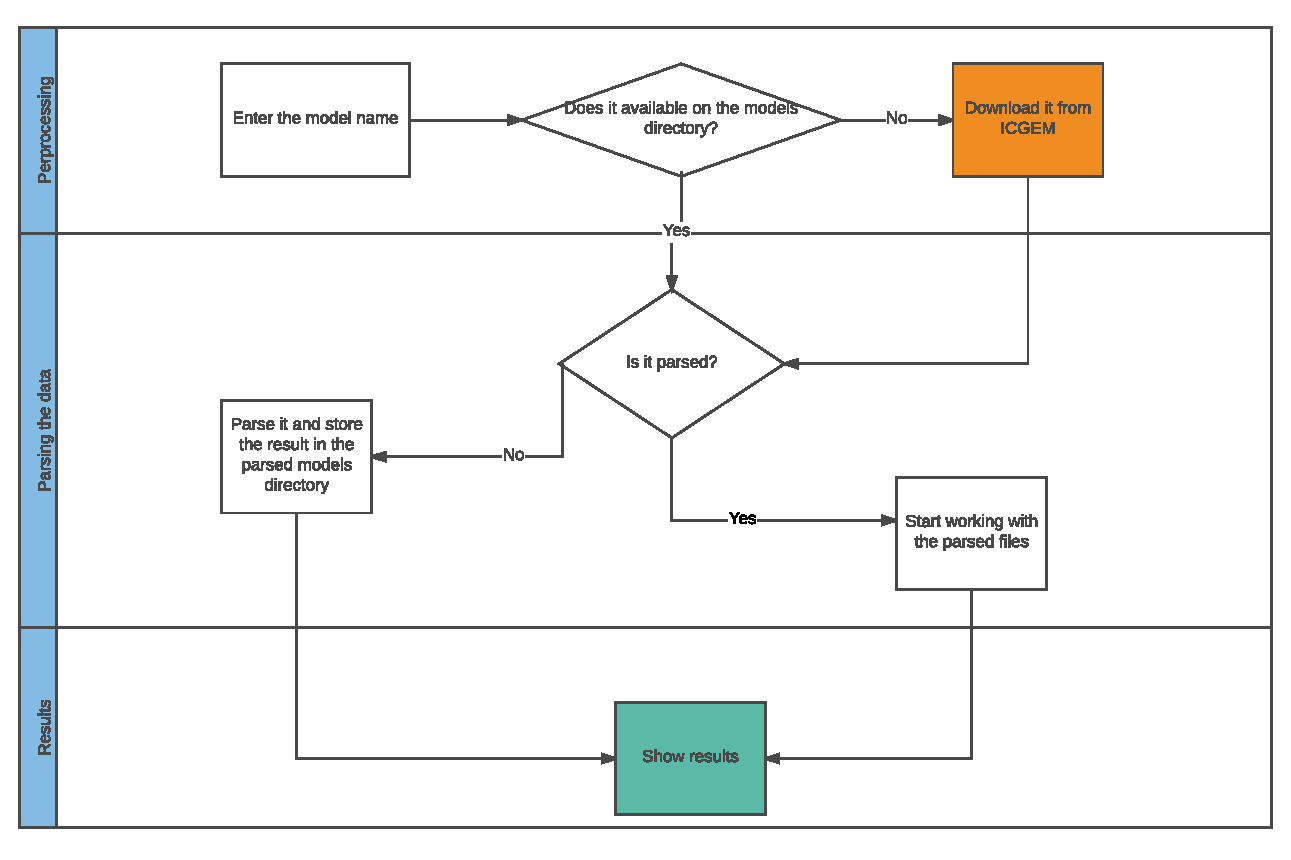
\includegraphics[scale=0.5]{Figures/cropped_flow.pdf}
	\centering
\end{figure}

GeoidApp also consists of advanced data analysis tools to help the users get the best out of their models. For each parsed model, GeoidApp creates a directory for that model and stores a log file that logs the result e.g., std and difference, and a *.csv files to store the results in a way that can easily be parsed later. GeoidApp also provides figures for each model being parsed. Another distinct feature is the interactive visualization for the result. This feature comes with the online version of GeoidApp \href{https://geoidapp.github.io}.
\\
The website of GeoidApp has many resources that cover different aspect of GeoidApp. A comprehensive documentation about the application, interactive visualizations, case studies results will all be presented at the website.
 

 % Experiment 1

\chapter{Results and Discussions}
We have evaluated different models in two types of datasets. The first data collected by \citep{adam} consists of 46 points. They use astrogeodetic observation to compute the geoid height. GPS/leveling data consists of 24 points collected during 2005-2008. We evaluated our models in different range of degrees (step of 5 degrees for EGM2008 and GECO, step of one degree for ITU\_GGC16 and ITU\_GRACE16). We used standard deviation as a measure of accuracy.

\section{Evaluation on astrogeodetic data}

Our evaluation of GGM using astrogedetic data shows very interesting results. There is a huge difference between GGM results and data of \citep{adam}. 


  \begin{table}[]
  	\centering
  	\caption{Top 5 degrees for model ITU\_GGC16}
  	\label{table:ggm_models}
  	\begin{tabular}{@{}lll@{}}
  		\toprule
  		\emph{degree} & std $\sigma$ [m]  & difference\\ \midrule
  		12 & 5.86797 &-10.7197\\
  		13 & 6.232&-10.0005\\
  		14 & 6.575&-9.9920\\
  		15 & 6.62&9.8420\\
  		11 & 6.74&-10.6067\\
  		121 & 6.758&-11.0029\\ \bottomrule  		
  	\end{tabular}
  \end{table}
  
    \begin{table}[]
    	\centering
    	\caption{Top 5 degrees for model EGM2008}
    	\label{table:ggm_models_egm2008}
    	\begin{tabular}{@{}lll@{}}
    		\toprule
    		\emph{degree} & std $\sigma$ [m]  & difference\\ \midrule
    		14 &6.57797646 &10.01617876\\
    		1722& 6.72616231& 11.10208562\\
    		1726 &6.72836585 &-11.10328207\\
    		1595 &6.73249422 &-11.10455418\\
    		1731 &6.73263864 &-11.10572496 \\ \bottomrule
    		
    	\end{tabular}
    \end{table}
    
    \begin{table}[]
    	\centering
    	\caption{Top 5 degrees for model EIGEN-6C4}
    	\label{table:ggm_models}
    	\begin{tabular}{@{}lll@{}}
    		\toprule
    		\emph{degree} & std $\sigma$ [m]  & difference\\ \midrule
    		
    		1729 &6.71829049 &-11.0980582\\
    		1718 &6.72207977 &-11.10011044\\
    		1609 &6.72228078 &-11.09995271\\
    		1598 &6.72349438 &-11.09978464\\
    		1872 & 6.72480567 & -11.10075124\\ \bottomrule
    		
    	\end{tabular}
    \end{table}
    
    
      \begin{table}[]
      	\centering
      	\caption{Top 5 degrees for model GECO}
      	\label{table:ggm_models_geco}
      	\begin{tabular}{@{}lll@{}}
      		\toprule
      		\emph{degree} & std $\sigma$ [m]  & difference\\ \midrule
      		10 & 7.7916 & -11.476 \\
      		14 &6.579  &-10.016 \\
      		18 &7.3629 &-10.144 \\
      		23 &7.5549 &-11.196 \\
      		27 &6.9829 &-10.997\\ \bottomrule
      		
      	\end{tabular}
      \end{table}
    
    
      \begin{table}[]
      	\centering
      	\caption{Top 5 degrees for model ITU\_GRACE16}
      	\label{table:ggm_models_itu_grace}
      	\begin{tabular}{@{}lll@{}}
      		\toprule
      		\emph{degree} & std $\sigma$ [m]  & difference\\ \midrule
      		12  &   5.8679769 &  -10.7196877\\
      		13  &  6.23255147 & -10.000530\\
      		14  & 6.57485872 &  -9.992074\\
      		15  & 6.61925941  & -9.84207\\
      		120 & 6.73941682 & -10.9837\\ \bottomrule
      		
      	\end{tabular}
      \end{table}
      
      
      \begin{figure}[t]
      	\caption{std behaviour with the change of degrees}
      	\label{egm2008_figure}
      	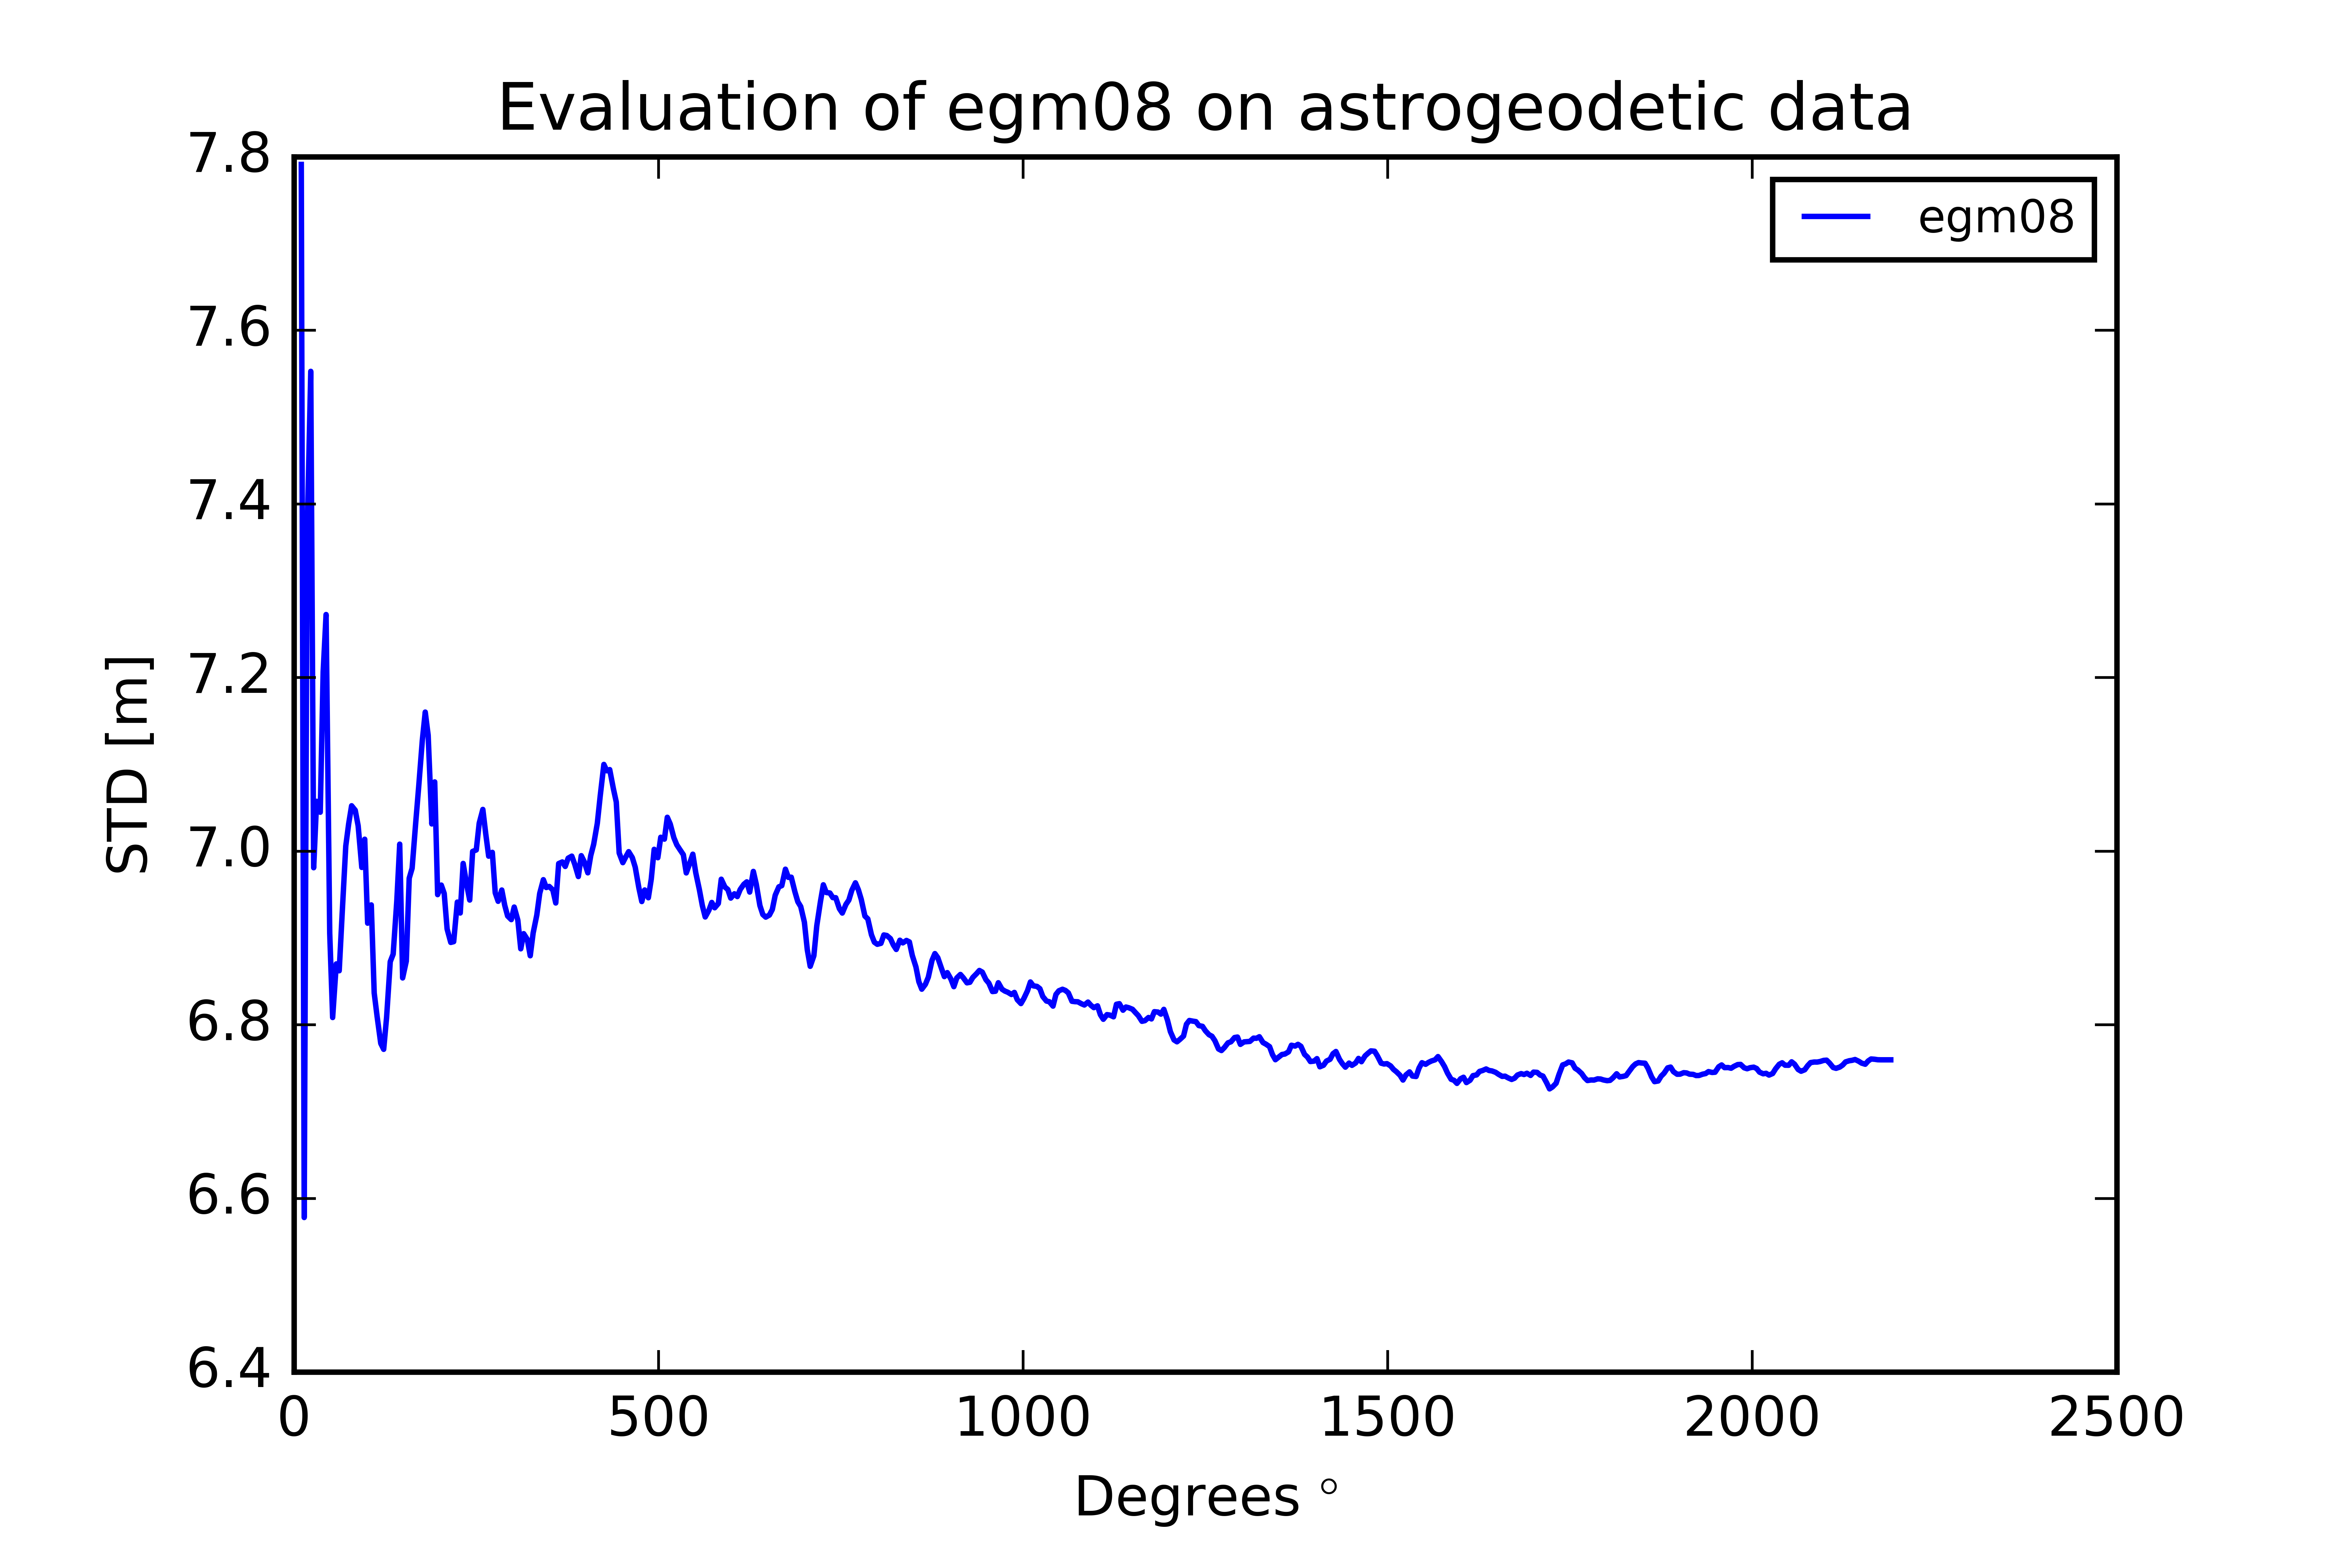
\includegraphics{Figures/egm08_figure.png}
      	\centering
      \end{figure}
      
      
      \begin{figure}[t]
      	\caption{std behaviour with the change of degrees}
      	\label{itu_grace16_figure}
      	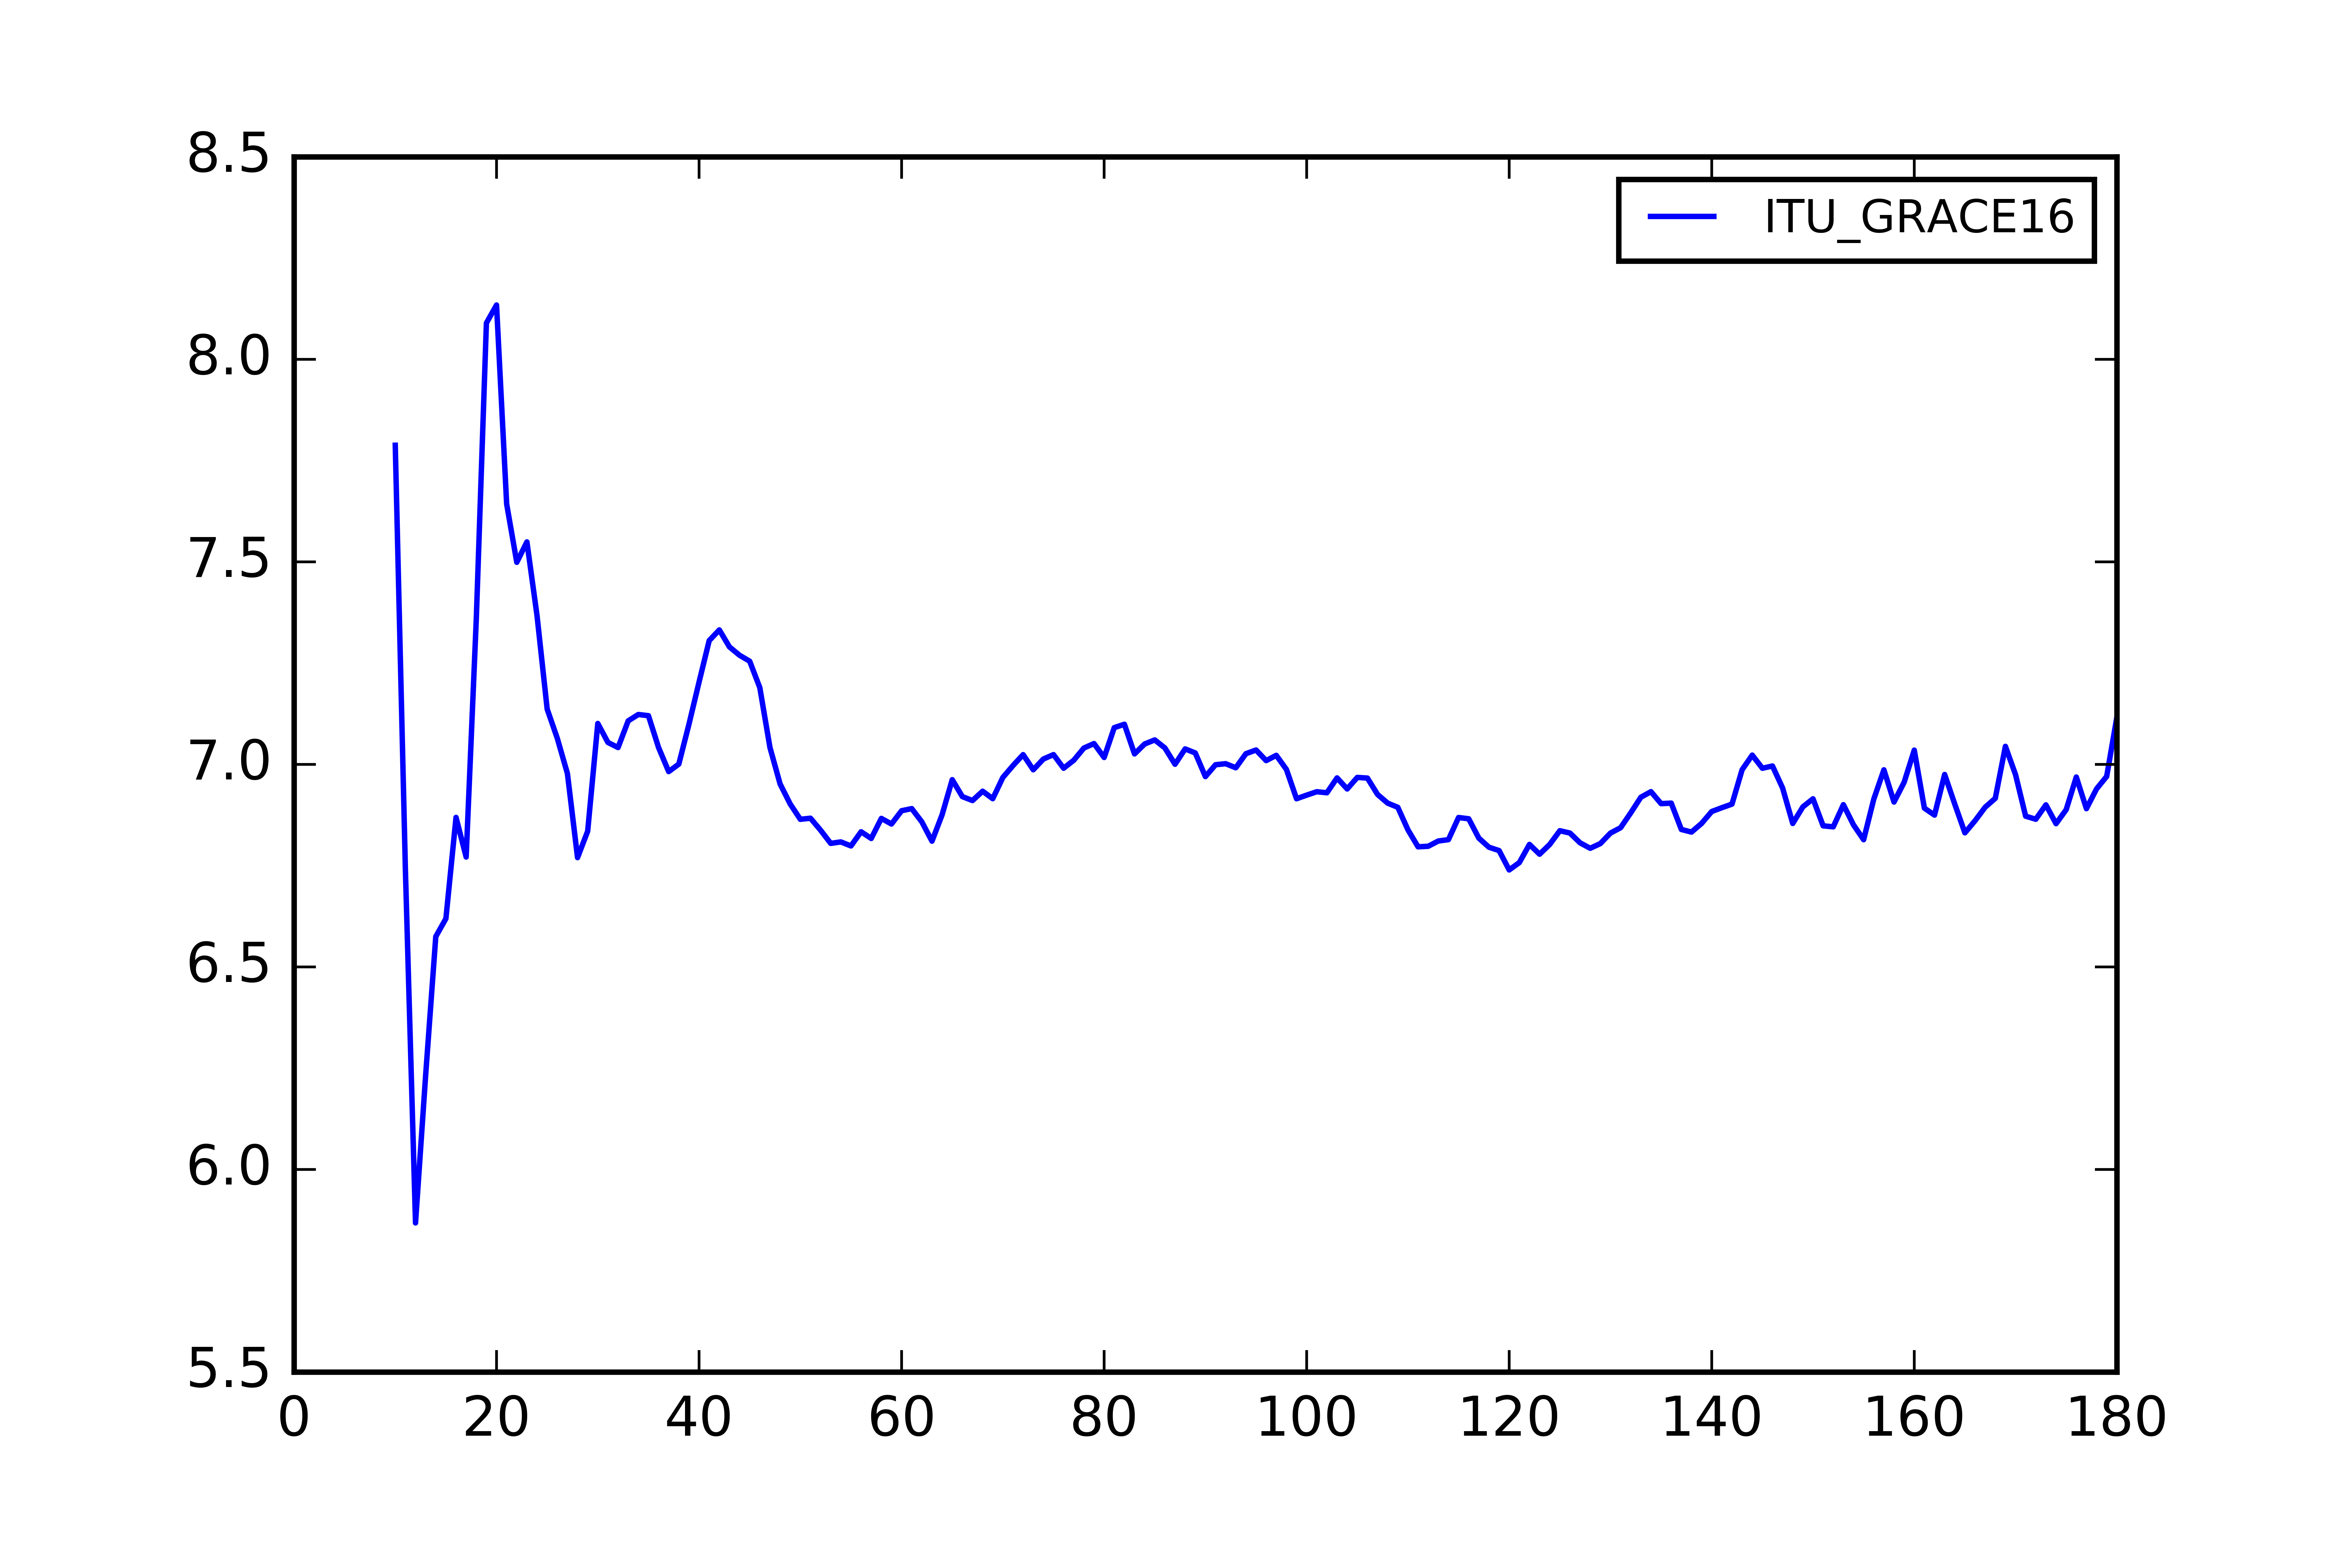
\includegraphics{Figures/ITU_GRACE16_figure.png}
      	\centering
      \end{figure}
      
      
      \begin{figure}[t]
      	\caption{std behaviour with the change of degrees}
      	\label{itu_ggc16_figure}
      	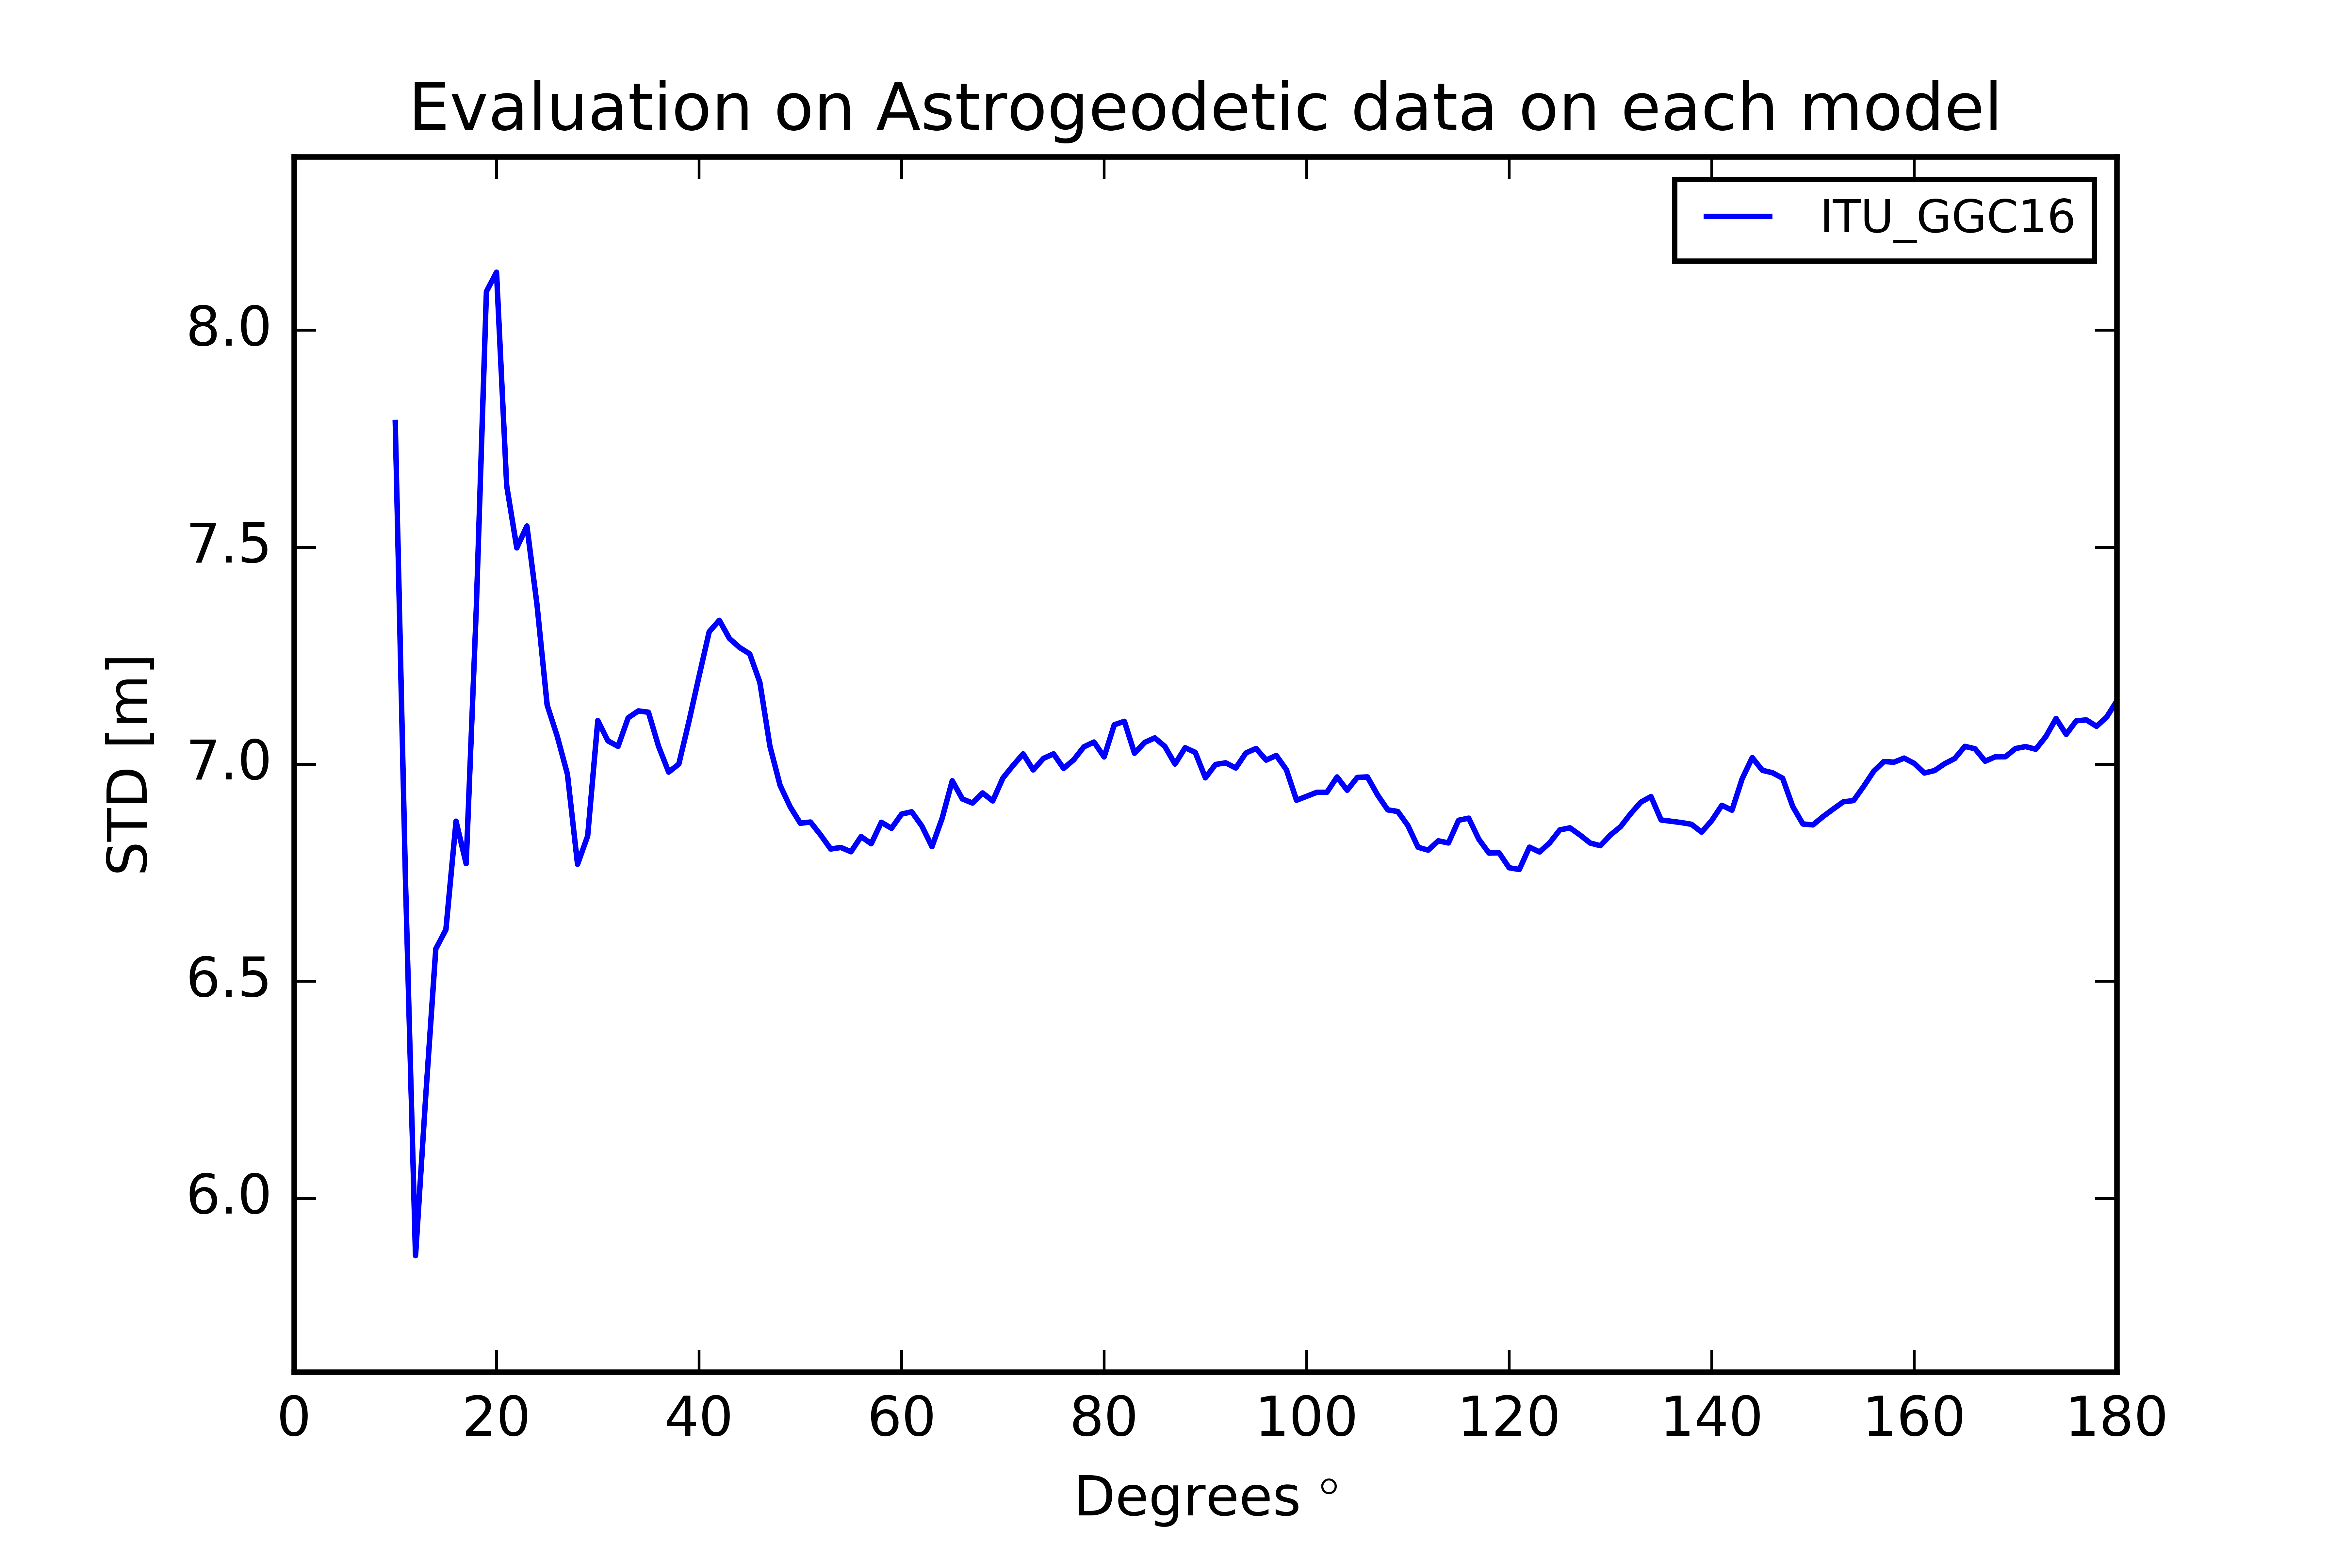
\includegraphics{Figures/ITU_GGC16_figure.png}
      	\centering
      \end{figure}
      
      
      \begin{figure}[t]
      	\caption{std behaviour with the change of degrees}
      	\label{geco_figure}
      	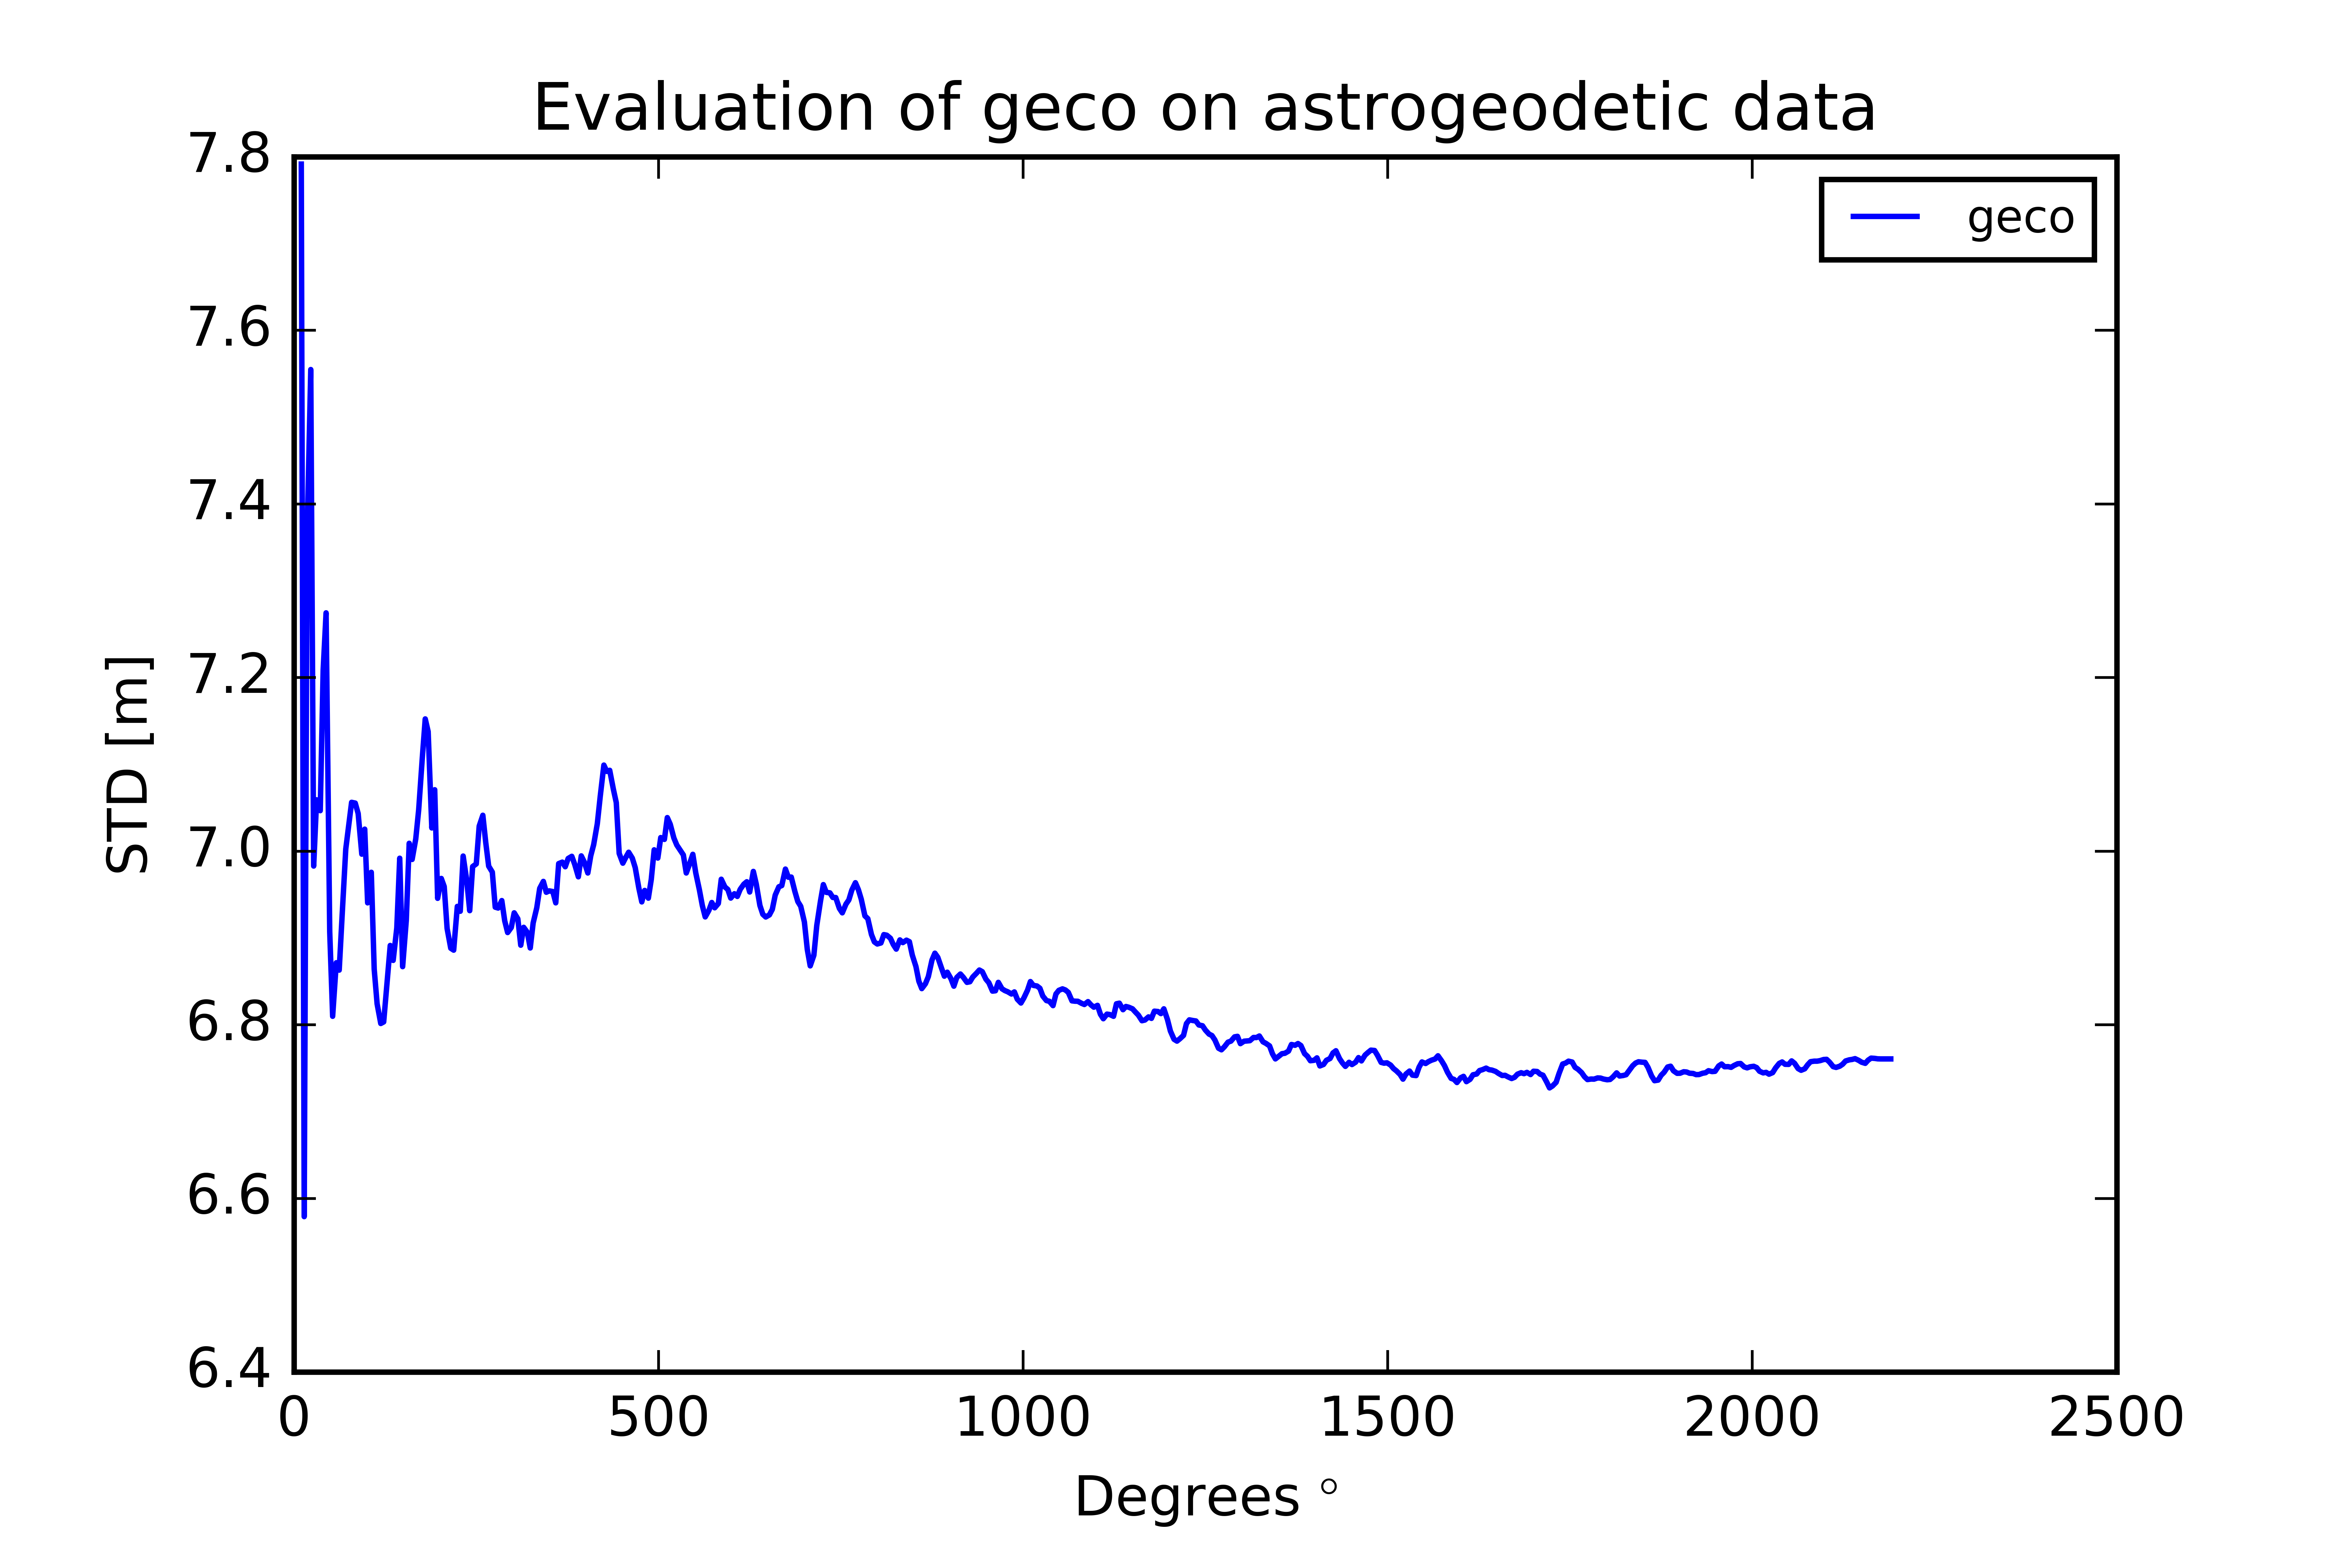
\includegraphics{Figures/geco_figure.png}
      	\centering
      \end{figure}
      
      \begin{figure}[t]
      	\caption{std behaviour with the change of degrees}
      	\label{eigen_6c4_figure}
      	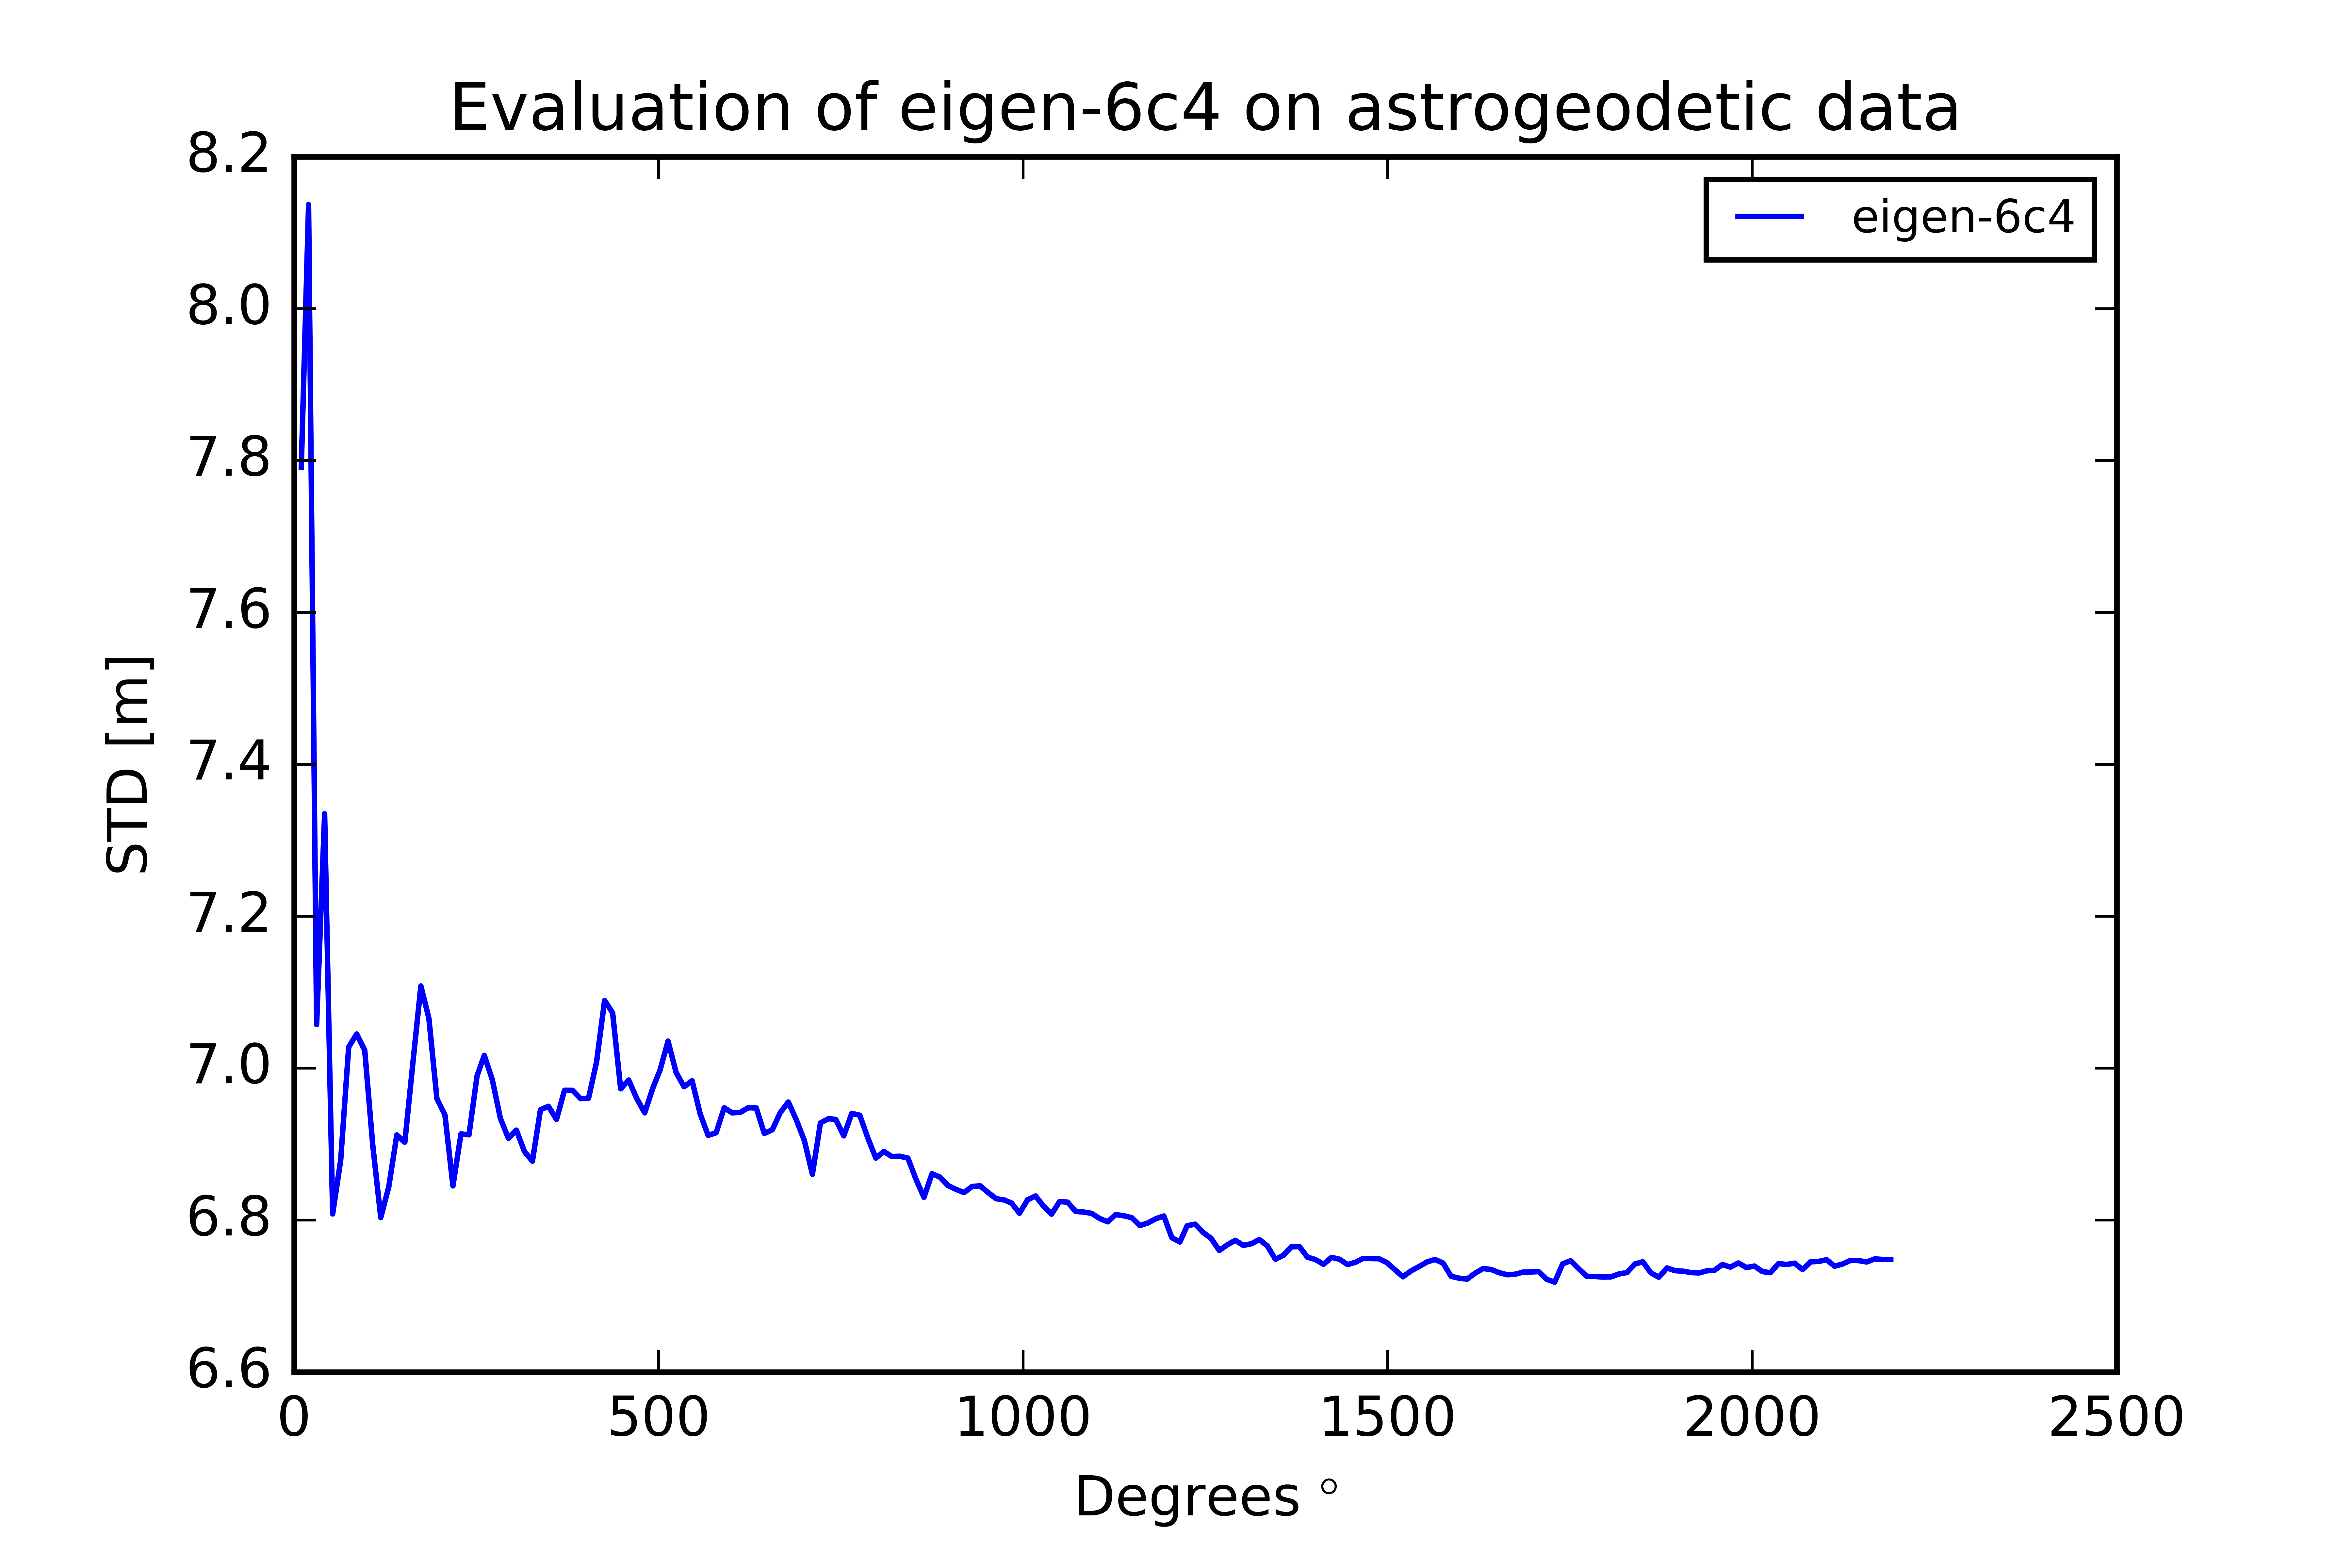
\includegraphics{Figures/eigen-6c4_figure.png}
      	\centering
      \end{figure} % Experiment 2

\chapter{Conclusion and Recommendations}
\label{Chapter6}

In this study we attempted to evaluate recent GRACE/GOCE models on Sudan. Our aim of this study was never to develop a new datum for Sudan, but rather to exhaustively try different models on our study area. Interestingly, our results--even without any corrections--are comparable to that reported by \citep{ahmed_msc, godah}. 

\begin{itemize}
	\item We begun our study by collecting terrestrial data for our study area
	\item GeoidApp: A software application that is mainly developed to help researchers evaluate different degrees of the model. The whole process is fully automated.
	\item The whole process of visualization, statistical analysis, reports are all handled within GeoidApp, and stored in their corresponding directories.
\end{itemize}

\section{Recommendations}

We believe that GGMs are the way to go for gravity field measurements. The traditional techniques for measuring gravity field has reached their intrinsic limitations. GGM provide global, regular and dense datasets of high and homogeneous quality. The use of GGM will lead, eventually, to the replace of expensive and time consuming spririt leveling, with the new fast, very cheap GPS/leveling. It will also contribute to the goal of unifying the regional datums.
\\
The availability of the data is a huge problem, in terms of the large un-surveyed areas, and also the access of the data. We have contacted with GETECH to get a copy of their data about Sudan, but they did not respond (as for the time we are writing this). We highly recommend to establish new GPS/leveling networks, that has more density and well distributed among Sudan. We do not recommend to use the dataset from \citep{osman} as it shows huge error compared to all of our models. 
\\
We, the authors of GeoidApp are very welcome to the use of our application in any research. We believe that our work will help researcher around the world to experiment with many different degrees of their GGMs without the need to manually tune any thing. We also highly recommend researchers to work on ``the unified datum"--geodetic main problem--which can only be solved by the means of GGM. The extreme low-cost of GPS leveling, and their speed should encourage researchers and government agencies to work even harder towards 1-cm precision model.  % Results and Discussion

%\input{Chapters/Chapter7} % Conclusion

%% ----------------------------------------------------------------
% Now begin the Appendices, including them as separate files

\addtocontents{toc}{\vspace{2em}} % Add a gap in the Contents, for aesthetics

\appendix % Cue to tell LaTeX that the following 'chapters' are Appendices

\chapter{Our Datasets}
In this appendix we show the complete datasets that we used in our study. Table \ref{complete_astrodata} shows the full dataset of \cite{osman}. The NaN value indicates a missing value.
% Please add the following required packages to your document preamble:
% \usepackage{booktabs}
\begin{table}[]
	\centering
	\caption{Complete astrogeodetic data of \cite{osman}}
	\label{complete_astrodata}
	\begin{tabular}{@{}lll@{}}
		\toprule
		latitutde & longitude & geoid height \\ \midrule
		22.169    & 31.489    & 10.000       \\
		20.136    & 30.662    & 9.556        \\
		18.473    & 30.840    & 10.198       \\
		17.051    & 31.272    & 10.199       \\
		14.496    & 30.251    & 14.180       \\
		13.832    & 29.654    & 15.833       \\
		13.233    & 30.110    & 15.354       \\
		12.866    & 29.956    & 15.647       \\
		12.776    & 30.853    & 14.453       \\
		11.604    & 30.411    & 15.387       \\
		10.823    & 31.113    & 14.851       \\
		10.279    & 30.980    & 15.346       \\
		10.247    & 31.067    & 15.188       \\
		8.619     & 31.402    & 15.332       \\
		7.071     & 31.319    & 13.970       \\
		5.805     & 31.783    & 11.396       \\
		4.701     & 31.779    & 14.180       \\
		14.840    & 34.088    & 12.449       \\
		15.511    & 36.253    & 12.683       \\
		16.615    & 36.254    & 12.745       \\
		17.593    & 36.038    & 11.665       \\
		18.710    & 37.102    & 6.847        \\
		19.501    & 37.260    & 6.133        \\
		20.337    & 37.107    & 7.051        \\
		21.087    & 37.107    & 6.440        \\
		22.314    & 36.513    & 9.930        \\
		22.541    & 35.894    & 12.432       \\
		15.526    & 32.582    & NaN          \\
		18.172    & 37.559    & 7.384        \\
		18.114    & 36.312    & 13.107       \\
		17.388    & 37.355    & 11.026       \\
		15.721    & 31.761    & 11.939       \\
		16.027    & 31.817    & 11.713       \\
		15.716    & 32.414    & 11.318       \\
		16.242    & 32.681    & 10.689       \\
		16.164    & 32.756    & 10.631       \\
		14.858    & 34.963    & 12.301       \\
		13.404    & 29.368    & 16.498       \\
		13.273    & 28.811    & 17.360       \\
		13.239    & 28.424    & 17.432       \\
		13.368    & 27.976    & 17.699       \\
		13.439    & 27.602    & 18.221       \\
		13.664    & 26.446    & 19.149       \\
		13.660    & 25.768    & 20.917       \\
		13.566    & 25.221    & 22.669       \\
		13.417    & 24.733    & 24.250       \\ \bottomrule
	\end{tabular}
\end{table}

% Please add the following required packages to your document preamble:
% \usepackage{booktabs}
\begin{table}[]
	\centering
	\caption{Full GPS/leveling dataset of Khartoum \citep{ahmed_msc}}
	\label{table:khartoum_gps_leveling_data}
	\begin{tabular}{@{}lll@{}}
		\toprule
		latitude & longitude & geoid height \\ \midrule
		16.172   & 32.153    & 3.573        \\
		15.822   & 32.313    & 2.998        \\
		15.890   & 32.684    & 3.619        \\
		16.077   & 32.722    & 3.119        \\
		15.811   & 33.087    & 2.175        \\
		15.809   & 32.900    & 2.285        \\
		15.613   & 32.808    & 2.020        \\
		16.352   & 31.965    & 4.174        \\
		15.848   & 32.517    & 3.078        \\
		16.119   & 32.531    & 2.263        \\
		15.992   & 32.340    & 3.210        \\
		15.810   & 32.154    & 3.210        \\
		16.113   & 31.965    & 3.197        \\
		15.993   & 32.901    & 3.254        \\
		15.988   & 32.144    & 3.447        \\
		15.470   & 33.080    & 2.297        \\
		15.651   & 32.388    & 2.810        \\
		15.721   & 32.514    & 2.655        \\
		16.139   & 32.638    & 2.420        \\
		15.607   & 32.518    & 2.673        \\
		15.599   & 32.108    & 2.538        \\
		15.524   & 32.577    & 2.599        \\
		15.259   & 32.555    & 2.231        \\
		15.340   & 32.394    & 2.692        \\ \bottomrule
	\end{tabular}
\end{table}

\section{Other models for Sudan using the rest of our GGM}
We show different models for Sudan using our GGM. While ITU\_GGC16 has scored the best result on our local data, the lack of the data, and the closeness of the results among the selected models make any of them a good candidate. The figures below are all purely from satellite observations, i.e., we did not use any local data to produce them. All of these models were evaluated using the maximum degree.
\\  
Figure \ref{figure:point_astro_dist} clearly shows the lack of our local data, and in the inhomogeneity in their distribution.

      \begin{figure}[t]
      	\caption{Points distribution of \cite{osman}}
      	\label{figure:point_astro_dist}
      	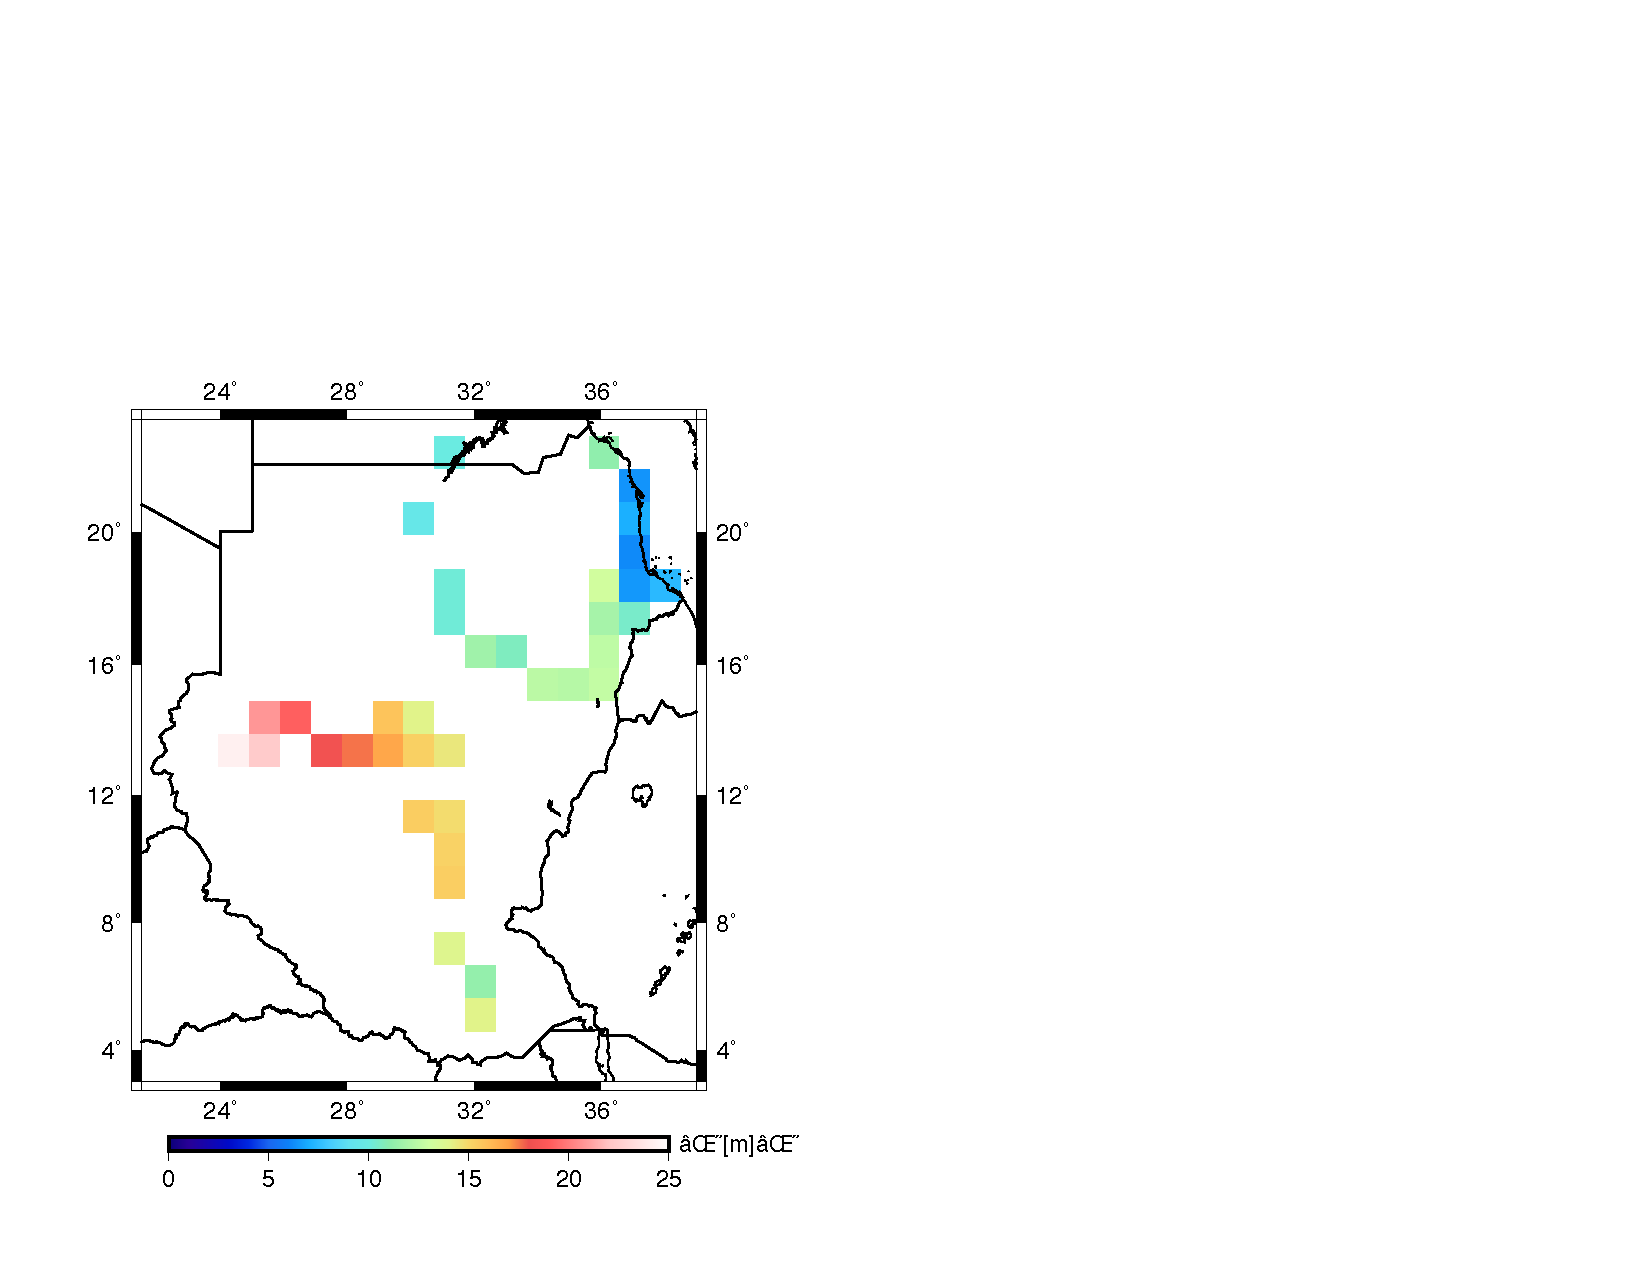
\includegraphics{Figures/points_astro_dist.pdf}
      	\centering
      \end{figure}
      
    \begin{figure}[t]
          	\caption{Points distribution of \cite{ahmed_msc}}
          	\label{figure:point_gps_dist}
          	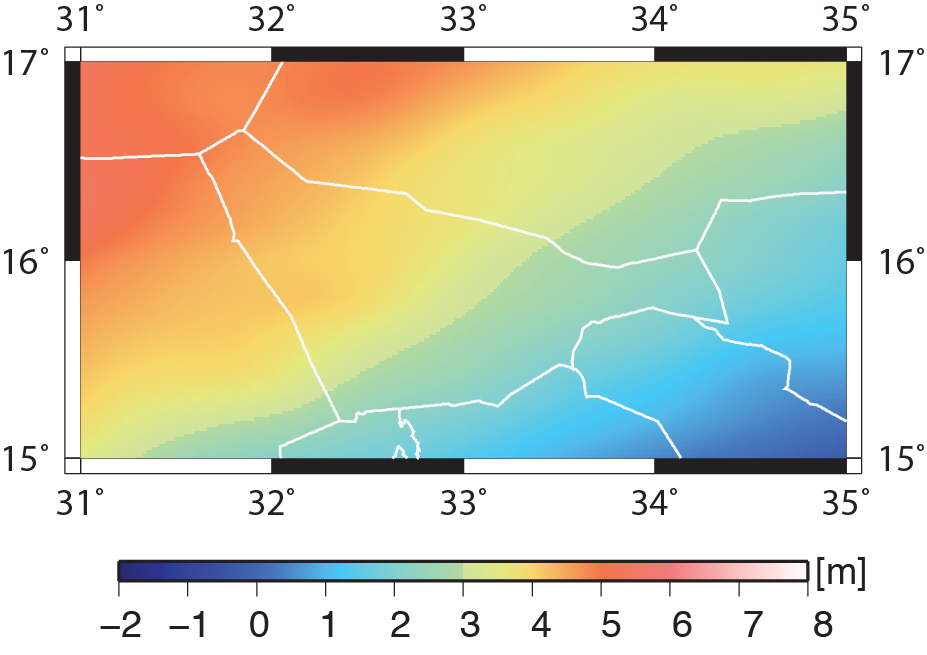
\includegraphics{Figures/krt.png}
          	\centering
    \end{figure}
    
        \begin{figure}[t]
        	\caption{New Geoid for Sudan based on EGM2008}
        	\label{figure:datum_egm2008}
        	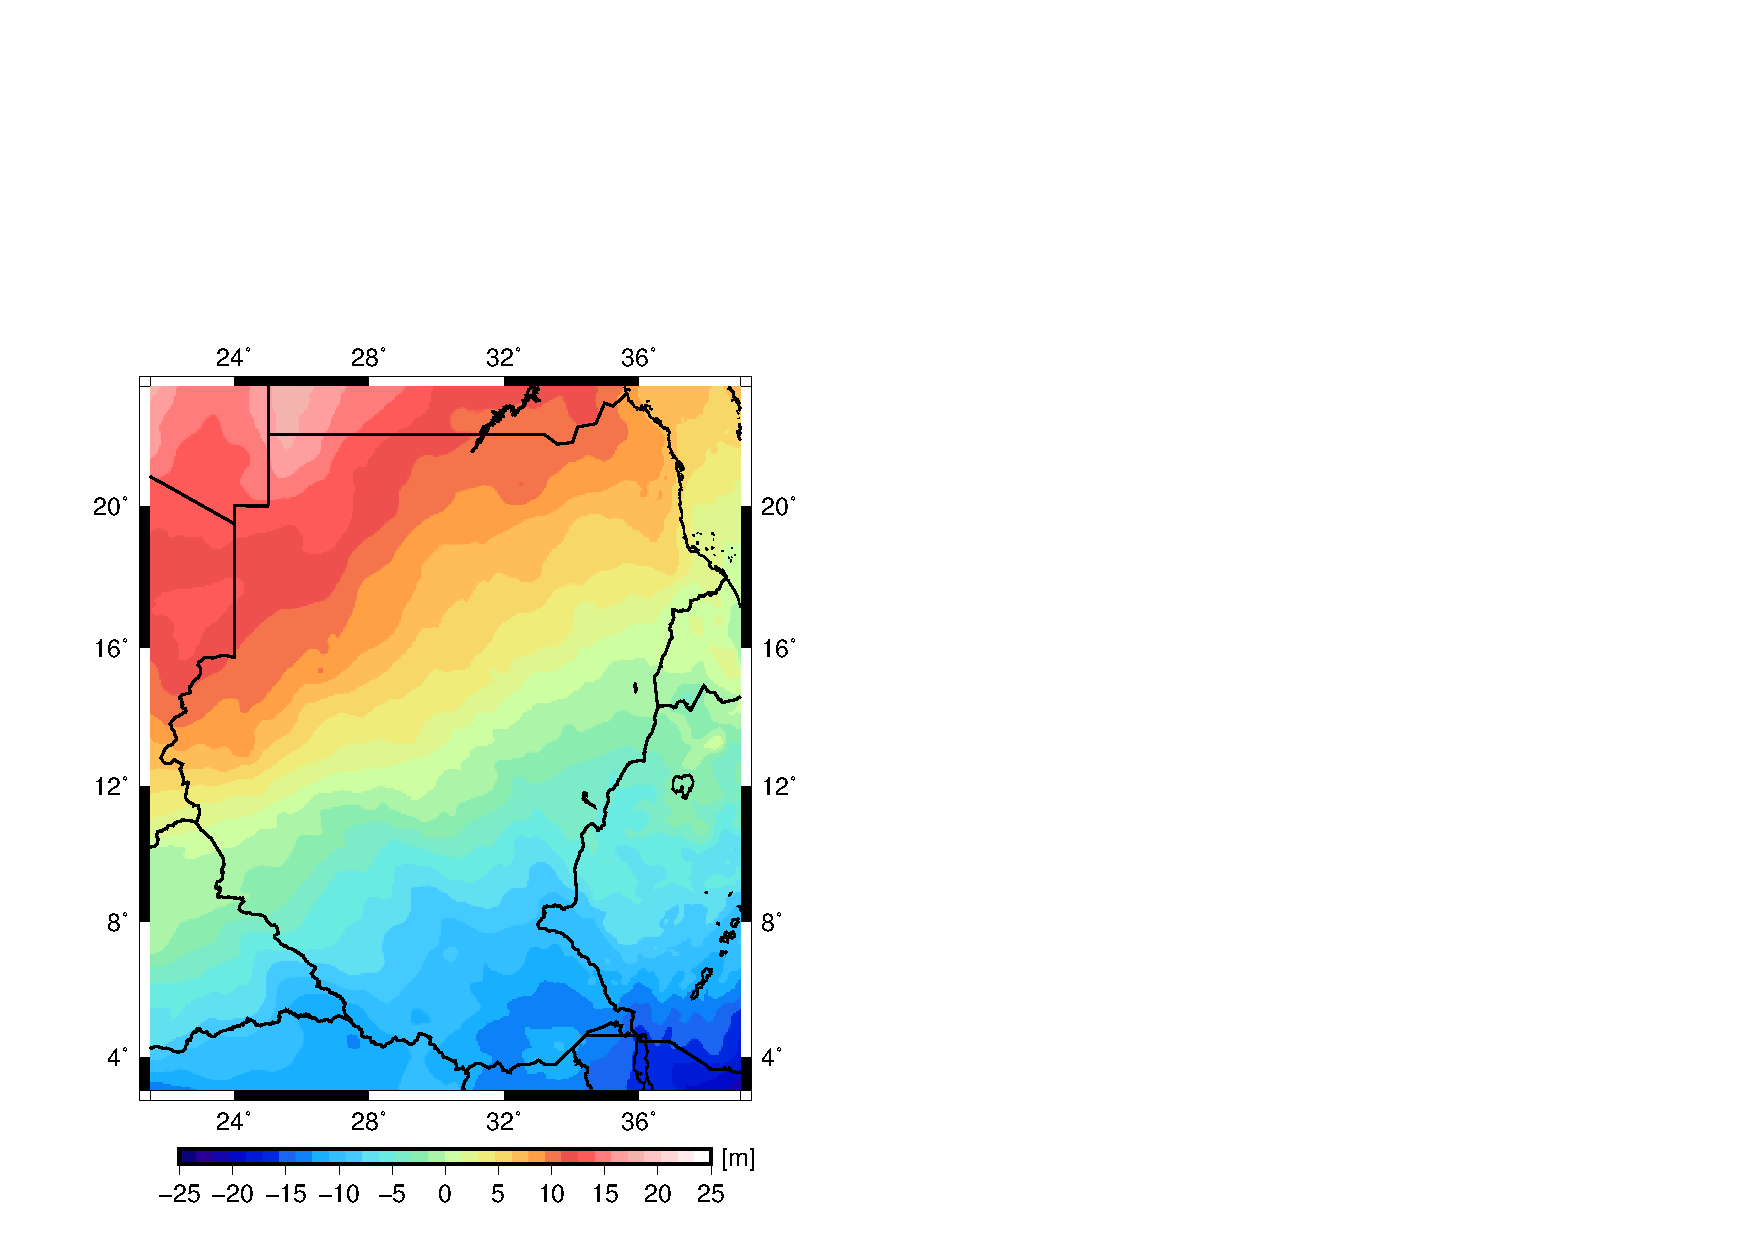
\includegraphics{Figures/cropped_egm2008.pdf}
        	\centering
        \end{figure}
        
        \begin{figure}[t]
              	\caption{New Geoid for Sudan based on EIGEN-6C4}
              	\label{figure:datum_eigen6c4}
              	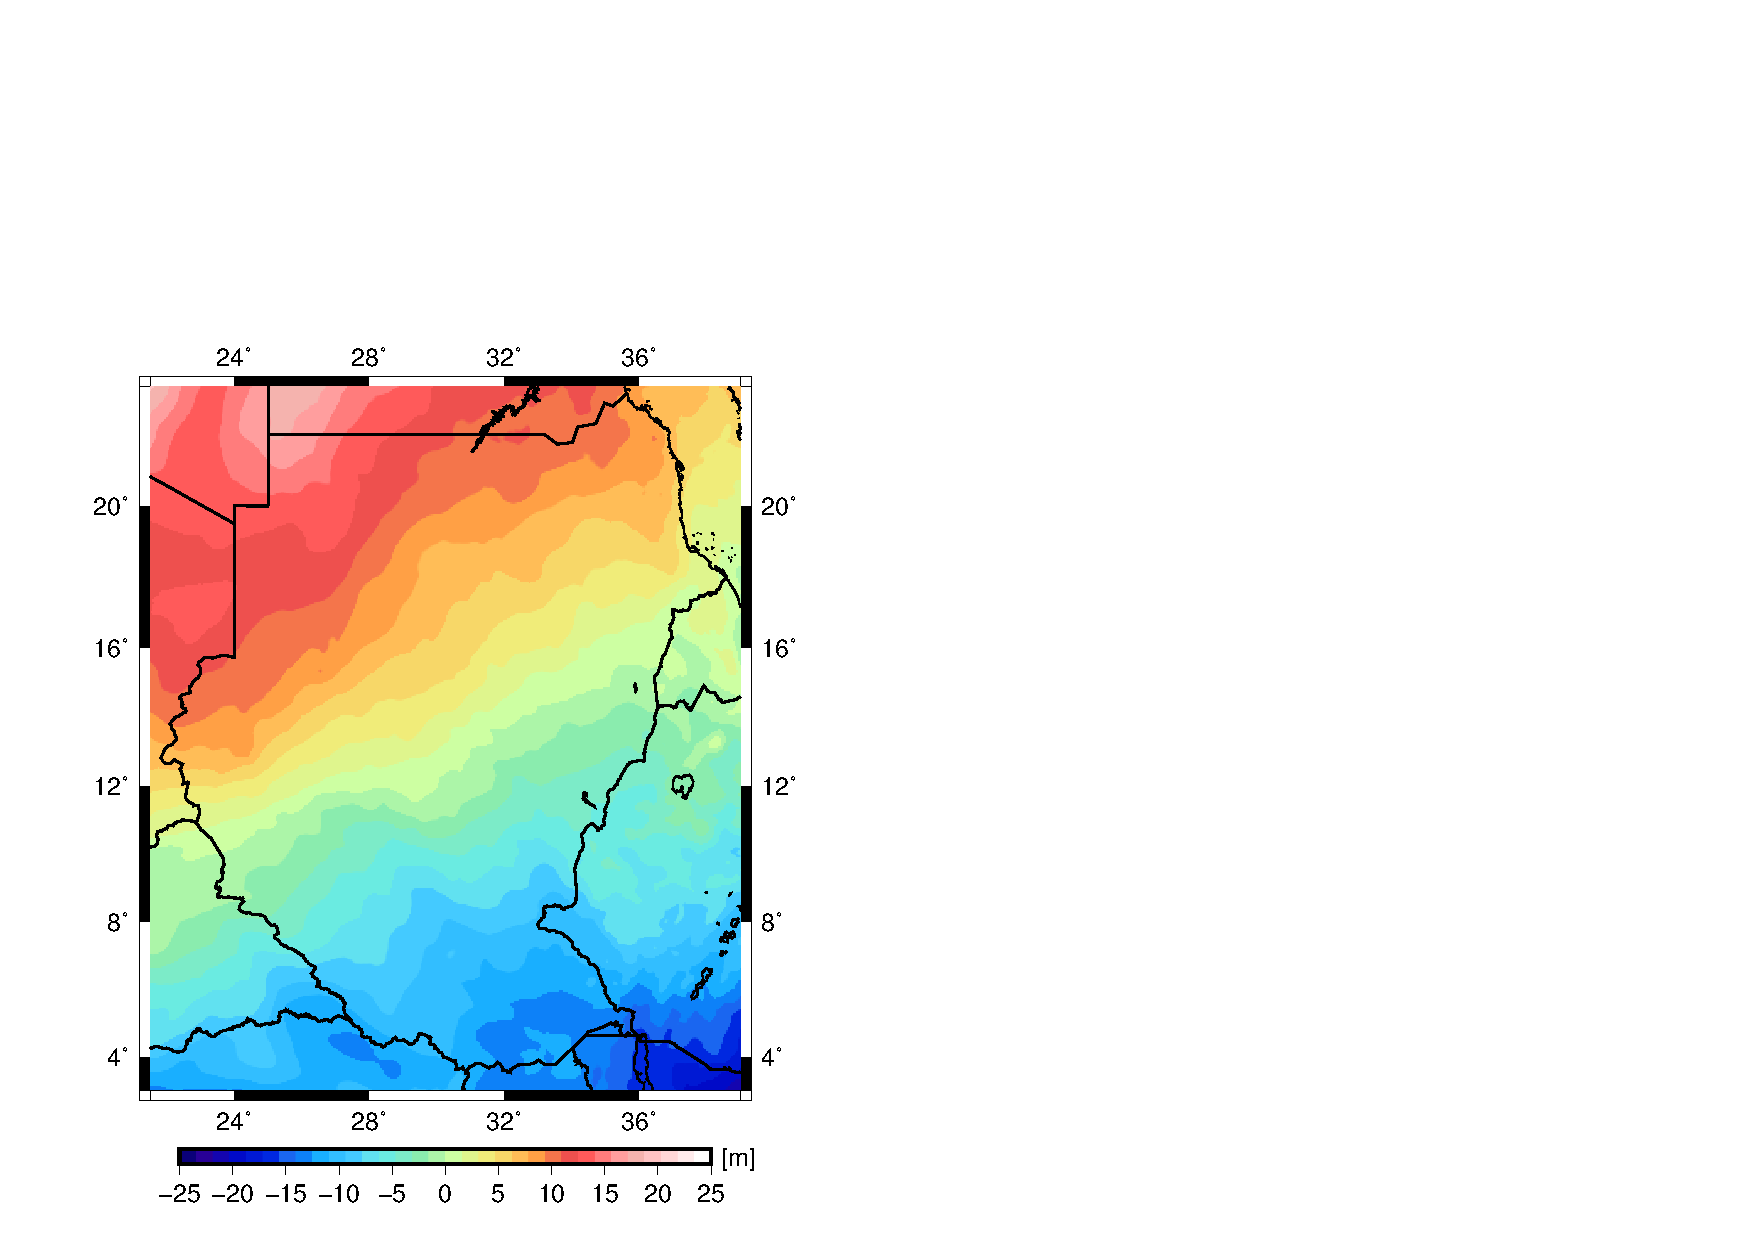
\includegraphics{Figures/cropped_eigen6c4.pdf}
              	\centering
        \end{figure}
        
            \begin{figure}[t]
                  	\caption{New Geoid for Sudan based on GECO}
                  	\label{figure:datum_geco}
                  	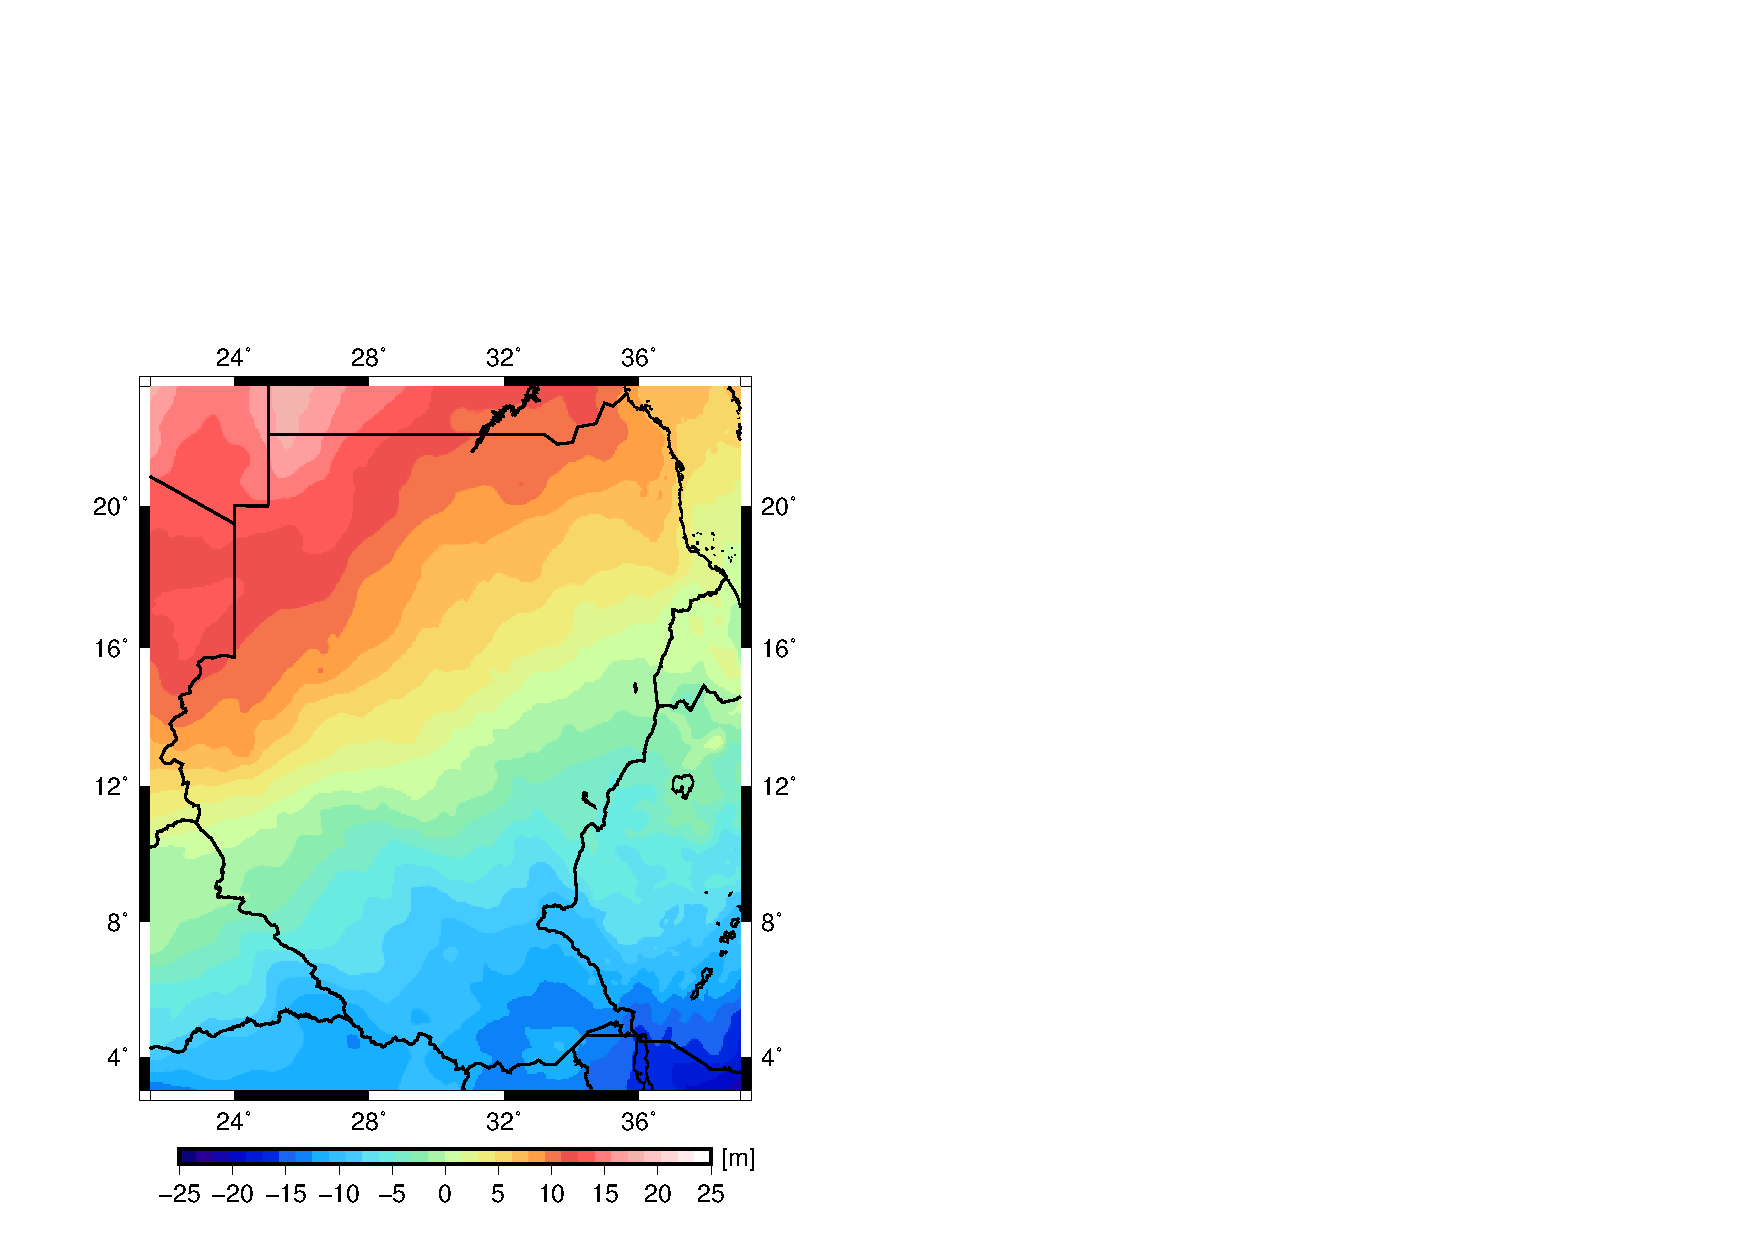
\includegraphics{Figures/cropped_geco.pdf}
                  	\centering
            \end{figure}
            
On Fig. \ref{figure:datum_itugrace16}, it is clear that ITU\_GRACE16 has a different behavior than other models. They \cite{itugrace16} reported that ITU\_GRACE16 is not regularized or constrained in any way, the errors increase with degree.Hence, they don't recommend to use it in any work without smoothing. 
                    \begin{figure}[t]
                       	\caption{New Geoid for Sudan based on ITU\_GRACE16}
                       	\label{figure:datum_itugrace16}
                       	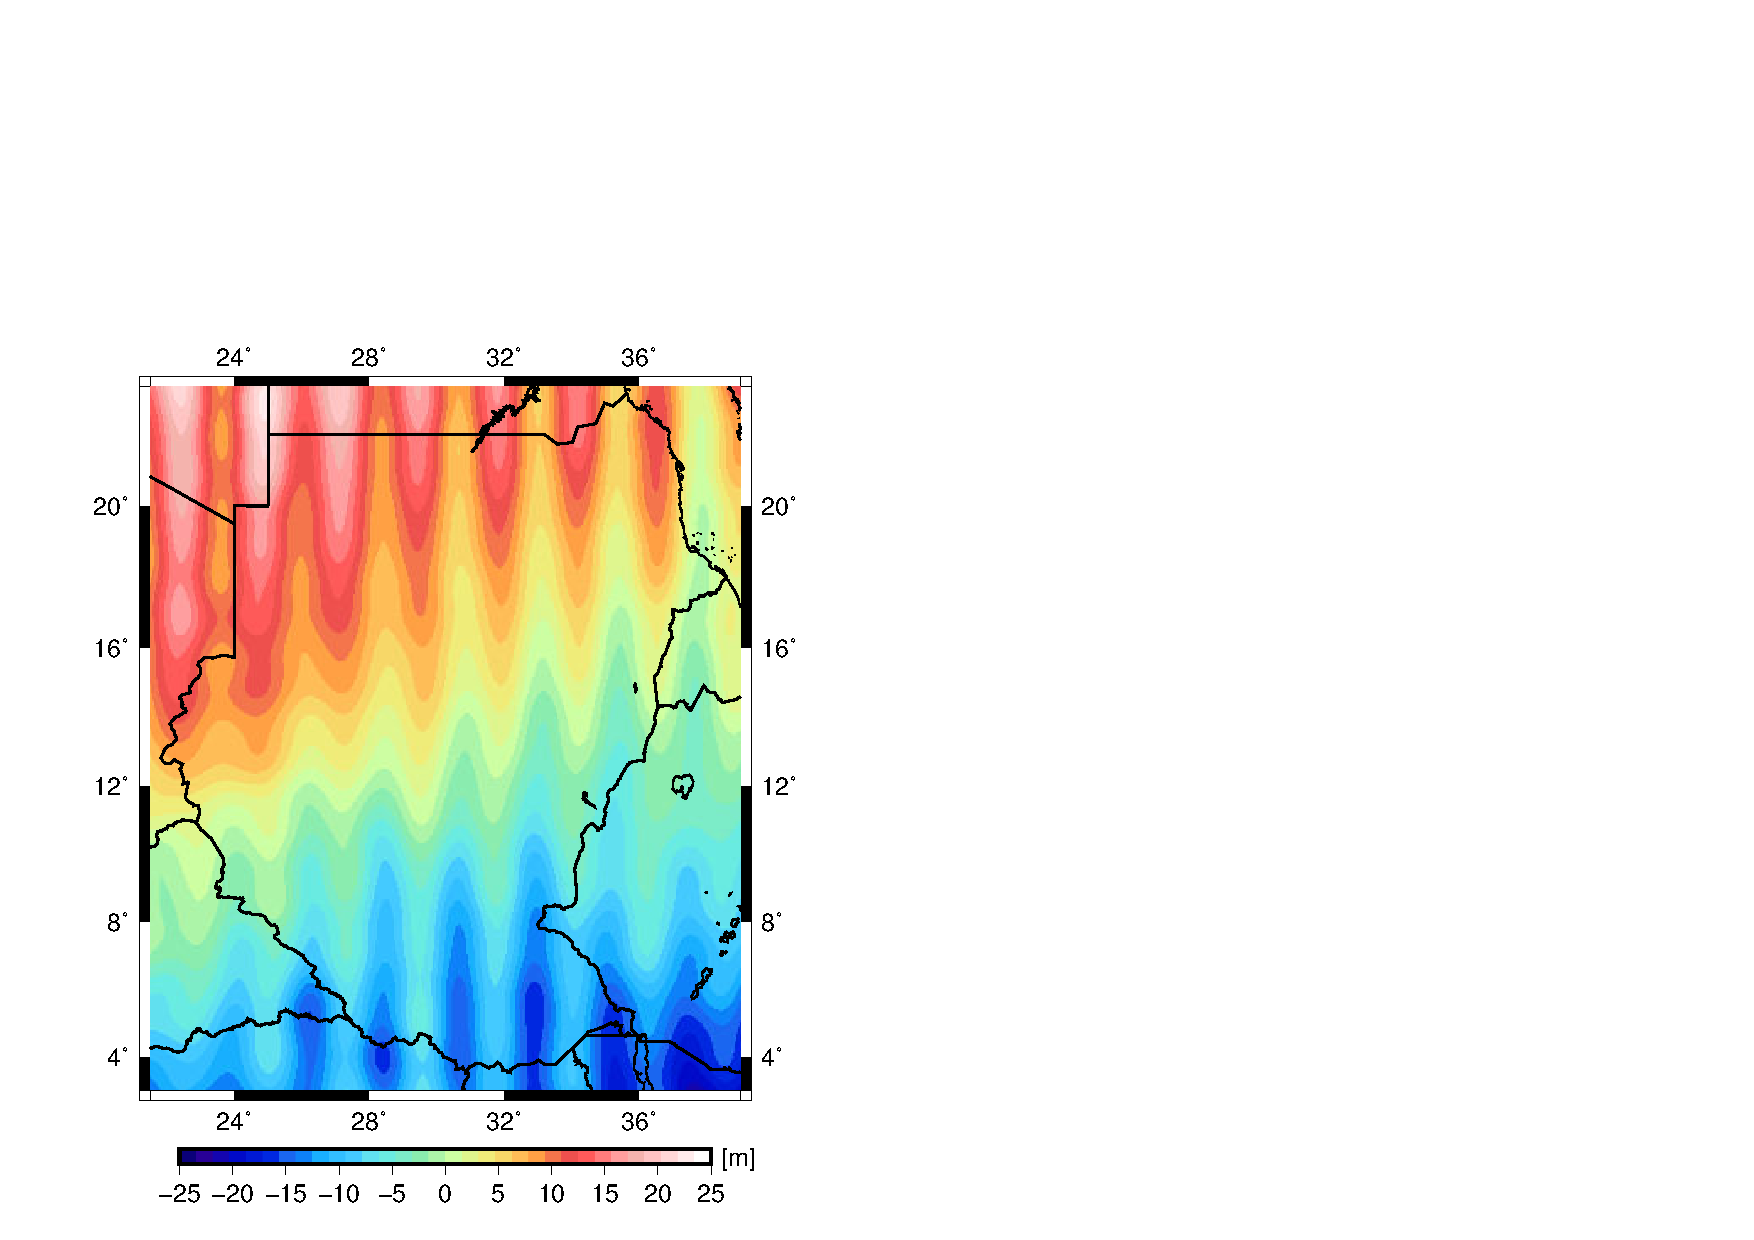
\includegraphics{Figures/cropped_itu_grace16.pdf}
                       	\centering
                    \end{figure}	% Appendix Title

%\input{Appendices/AppendixB} % Appendix Title

%\input{Appendices/AppendixC} % Appendix Title

\addtocontents{toc}{\vspace{2em}}  % Add a gap in the Contents, for aesthetics
\backmatter

%% ----------------------------------------------------------------
\label{Bibliography}
\lhead{\emph{Bibliography}}  % Change the left side page header to "Bibliography"
\bibliographystyle{unsrtnat}  % Use the "unsrtnat" BibTeX style for formatting the Bibliography
\bibliography{Bibliography}  % The references (bibliography) information are stored in the file named "Bibliography.bib"

\end{document}  % The End
%% ----------------------------------------------------------------